%Version 3 October 2023
% See section 11 of the User Manual for version history
%
%%%%%%%%%%%%%%%%%%%%%%%%%%%%%%%%%%%%%%%%%%%%%%%%%%%%%%%%%%%%%%%%%%%%%%
%%                                                                 %%
%% Please do not use \input{...} to include other tex files.       %%
%% Submit your LaTeX manuscript as one .tex document.              %%
%%                                                                 %%
%% All additional figures and files should be attached             %%
%% separately and not embedded in the \TeX\ document itself.       %%
%%                                                                 %%
%%%%%%%%%%%%%%%%%%%%%%%%%%%%%%%%%%%%%%%%%%%%%%%%%%%%%%%%%%%%%%%%%%%%%

%%\documentclass[referee,sn-basic]{sn-jnl}% referee option is meant for double line spacing

%%=======================================================%%
%% to print line numbers in the margin use lineno option %%
%%=======================================================%%

%%\documentclass[lineno,sn-basic]{sn-jnl}% Basic Springer Nature Reference Style/Chemistry Reference Style

%%======================================================%%
%% to compile with pdflatex/xelatex use pdflatex option %%
%%======================================================%%

%%\documentclass[pdflatex,sn-basic]{sn-jnl}% Basic Springer Nature Reference Style/Chemistry Reference Style


%%Note: the following reference styles support Namedate and Numbered referencing. By default the style follows the most common style. To switch between the options you can add or remove “Numbered” in the optional parenthesis. 
%%The option is available for: sn-basic.bst, sn-vancouver.bst, sn-chicago.bst%  
 
%%\documentclass[sn-nature]{sn-jnl}% Style for submissions to Nature Portfolio journals
%%\documentclass[sn-basic]{sn-jnl}% Basic Springer Nature Reference Style/Chemistry Reference Style
\documentclass[sn-mathphys-num]{sn-jnl}% Math and Physical Sciences Numbered Reference Style 
%%\documentclass[sn-mathphys-ay]{sn-jnl}% Math and Physical Sciences Author Year Reference Style
%%\documentclass[sn-aps]{sn-jnl}% American Physical Society (APS) Reference Style
%%\documentclass[sn-vancouver,Numbered]{sn-jnl}% Vancouver Reference Style
%%\documentclass[sn-apa]{sn-jnl}% APA Reference Style 
%%\documentclass[sn-chicago]{sn-jnl}% Chicago-based Humanities Reference Style

%%%% Standard Packages
%%<additional latex packages if required can be included here>

\usepackage{graphicx}%
\usepackage{multirow}%
\usepackage{amsmath,amssymb,amsfonts}%
\usepackage{amsthm}%
\usepackage{mathrsfs}%
\usepackage[title]{appendix}%
\usepackage{xcolor}%
\usepackage{textcomp}%
\usepackage{manyfoot}%
\usepackage{booktabs}%
\usepackage{algorithm}%
\usepackage{algorithmicx}%
\usepackage{algpseudocode}%
\usepackage{listings}%
%%%%
\usepackage{anyfontsize}

%%%%%=============================================================================%%%%
%%%%  Remarks: This template is provided to aid authors with the preparation
%%%%  of original research articles intended for submission to journals published 
%%%%  by Springer Nature. The guidance has been prepared in partnership with 
%%%%  production teams to conform to Springer Nature technical requirements. 
%%%%  Editorial and presentation requirements differ among journal portfolios and 
%%%%  research disciplines. You may find sections in this template are irrelevant 
%%%%  to your work and are empowered to omit any such section if allowed by the 
%%%%  journal you intend to submit to. The submission guidelines and policies 
%%%%  of the journal take precedence. A detailed User Manual is available in the 
%%%%  template package for technical guidance.
%%%%%=============================================================================%%%%

%% as per the requirement new theorem styles can be included as shown below
%\theoremstyle{thmstyleone}%
\newtheorem{theorem}{Theorem}%  meant for continuous numbers
%%\newtheorem{theorem}{Theorem}[section]% meant for sectionwise numbers
%% optional argument [theorem] produces theorem numbering sequence instead of independent numbers for Proposition
\newtheorem{proposition}[theorem]{Proposition}% 
%%\newtheorem{proposition}{Proposition}% to get separate numbers for theorem and proposition etc.

%\theoremstyle{thmstyletwo}%
\newtheorem{example}{Example}%
\newtheorem{remark}{Remark}%

%\theoremstyle{thmstylethree}%
\newtheorem{definition}{Definition}%

\raggedbottom
%%\unnumbered% uncomment this for unnumbered level heads

\usepackage[acronym]{glossaries}

\makeglossaries
\newacronym{dst}{Dst}{Disturbance Storm-Time}
\newacronym{rin}{RIN}{The Royal Institute of Navigation}
\newacronym{ion}{ION}{The Institute of Navigation}
\newacronym{ursi}{URSI}{Union Radio-Scientifique Internationale}
\newacronym{rinex}{RINEX}{Receiver Independent Exchange Format}
\newacronym{tec}{TEC}{Total Electron Content}
\newacronym{dtec}{dTEC}{standard deviation of Total Electron Content}
\newacronym{gnss}{GNSS}{Global Navigation Satellite System}
\newacronym{pnt}{PNT}{Positioning, Navigation, and Timing}
\newacronym{svm}{SVM}{Support Vector Machine}
\newacronym{svn}{SVN}{Support Vector Network}
\newacronym{svc}{SVC}{Support Vector Clustering}
\newacronym{dt}{DT}{Decision Tree}
\newacronym{tdidt}{TDIDT}{Top-Down Induction of Decision Trees}
\newacronym{nb}{NB}{Naive Bayes}
\newacronym{ci}{CI}{Confidence Interval}
\newacronym{nir}{NIR}{No Information Rate}
\newacronym{nn}{NN}{Neural Network}
\newacronym{ann}{ANN}{Artificial Neural Network}
\newacronym{pls}{PLS}{Partial Least Squares}
\newacronym{pls-da}{PLS-DA}{Partial Least Squares Discriminant Analysis}
\newacronym{fda}{FDA}{Flexible Discriminant Analysis}
\newacronym{lda}{LDA}{Linear Discriminant Analysis}
\newacronym{pca}{PCA}{Principal Component Analysis}
\newacronym{manova}{MANOVA}{Multivariate Analysis Of Variance}
\newacronym{mars}{MARS}{Multivariate Adaptive Regression Splines}
\newacronym{nda}{NDA}{Normal Discriminant Analysis}
\newacronym{nas}{NAS}{Neural Architecture Search}
\newacronym{dbscan}{DBSCAN}{Density-Based Spatial Clustering}
\newacronym{cnn}{CNN}{Convolutional Neural Network}
\newacronym{rf}{RF}{Random Forest}
\newacronym{tp}{TP}{True Positive}
\newacronym{tn}{TN}{True Negative}
\newacronym{fp}{FP}{False Positive}
\newacronym{fn}{FN}{False Negative}
\newacronym{tpr}{TPR}{True Positive Rate}
\newacronym{tnr}{TNR}{True Negative Rate}
\newacronym{ppv}{PPV}{Positive Predictive Value}
\newacronym{npv}{NPV}{Negative Predictive Value}
\newacronym{dr}{DR}{Detection Rate}
\newacronym{dp}{DP}{Detection Prevalence}
\newacronym{ba}{BA}{Balanced Accuracy}
\newacronym{sar}{SAR}{Synthetic Aperture Radar}
\newacronym{cca}{CCA}{Canonical Correlation Analysis}
\newacronym{pod}{POD}{Proper Orthogonal Decomposition}
\newacronym{svd}{SVD}{Singular Value Decomposition}
\newacronym{eof}{EOF}{Empirical Orthogonal Functions}
\newacronym{evd}{EVD}{Eigenvalue Decomposition}
\newacronym{gps}{GPS}{Global Positioning System}
\newacronym{klt}{KLT}{Karhunen–Loève Theorem}
\newacronym{gpu}{GPU}{Graphics Processing Unit}
\newacronym{cpu}{CPU}{Central Processing Unit}
\newacronym{ram}{RAM}{Random Access Memory}
\newacronym{ml}{ML}{machine learning}
\newacronym{aa2}{(AA)2}{Ambient-Aware Application-Aligned}
\newacronym{tid}{TID}{Traveling Ionospheric Disturbance}
\newacronym{epb}{EPB}{Equatorial Plasma Bubbles}
\newacronym{gec}{GEC}{Global Electric Current}
\newacronym{spdf}{SPDF}{Space Physics Data Facility}
\newacronym{noaa}{NOAA}{National Oceanic and Atmospheric Administration}
\newacronym{swpc}{SWPC}{Space Weather Prediction Center}
\newacronym{nrcan}{NRCAN}{Natural Resources Canada}
\newacronym{gfz}{GFZ}{German Research Centre for Geosciences}
\newacronym{nasa}{NASA}{National Aeronautics and Space Administration}
\newacronym{euv}{EUV}{Extreme ultraviolet}

\begin{document}

\title[A $Dst$-based space weather conditions machine learning classification  model for GNSS PNT performance analysis]{A $Dst$-based space weather conditions machine learning classification  model for GNSS PNT performance analysis}

\author[1,2]{\fnm{Lucija} \sur{\v{Z}u\v{z}i\'{c}}}\email{lucija.zuzic@uniri.hr}
\equalcont{These authors contributed equally to this work.}

\author[1,2]{\fnm{Deni} \sur{Klen}}\email{deni.klen@uniri.hr}
\equalcont{These authors contributed equally to this work.}

\author[3]{\fnm{Teodor B.} \sur{Iliev}}\email{tiliev@uni-ruse.bg}

\author*[1,2,4]{\fnm{Renato} \sur{Filjar}}\email{renato.filjar@uniri.hr}

\affil*[1]{\orgdiv{Department of Computer Engineering}, \orgname{Faculty of Engineering, University of Rijeka}, \orgaddress{\street{Vukovarska 58}, \city{Rijeka}, \postcode{51000}, \country{Croatia}}}

\affil[2]{\orgdiv{Center for Artificial Intelligence and Cybersecurity}, \orgname{University of Rijeka}, \orgaddress{\street{Radmile Matejcic 2}, \city{Rijeka}, \postcode{51000}, \country{Croatia}}}

\affil[3]{\orgdiv{Department of Telecommunication}, \orgname{University of Ruse}, \orgaddress{\street{8 Studentska str.}, \city{Ruse}, \postcode{7017}, \country{Bulgaria}}}

\affil[4]{\orgdiv{Laboratory for Spatial Intelligence}, \orgname{Hrvatsko Zagorje Krapina University of Applied Sciences}, \orgaddress{\street{Setaliste hrvatskog narodnog preporoda 6}, \city{Krapina}, \postcode{49000}, \country{Croatia}}}

\abstract{Ambient conditions classification enables systematic mitigation of adversarial effects on the Global Navigation Satellite System (GNSS) Positioning, Navigation, and Timing (PNT) performance. This research contributes to the problem by proposing a classification model of space weather events for sub-equatorial regions. The proposed model uses machine learning-based classification applied to the experimental observations of geomagnetic field components, observed Total Electron Content ($TEC$), and Disturbance Storm-Time ($Dst$-index). A SVM with a Polynomial Kernel, C5.0 Decision Tree (DT), Naive Bayes (NB), shallow Neural Network (NN), Partial Least Squares (PLS), Flexible Discriminant Analysis (FDA), and shallow NN using Principal Component Analysis (PCA) was applied to develop the candidate model to classify observations of the geomagnetic field in $TEC$, combined with other variables, into one of the scenarios of space weather conditions. Performance is assessed using a confusion matrix and development time to yield the NB as the best performer. The proposed $Dst$-based classification model serves as an indicator of a geomagnetic/ionospheric storm in progress, thus alerting GNSS users of potential degradation in GNSS PNT performance and setting up a framework for the development of a tailored GNSS ionospheric correction model for specific classes of the space weather conditions.}

\keywords{Global Navigation Satellite System (GNSS) Positioning, Navigation, and Timing (PNT), space weather conditions, machine learning (ML), classification model, Decision Tree (DT), Neural Network (NN), sensor observations aggregation, geomagnetic field, Total Electron Content ($TEC$), Disturbance Storm-Time ($Dst$-index)}

%%\pacs[JEL Classification]{D8, H51}

%%\pacs[MSC Classification]{35A01, 65L10, 65L12, 65L20, 65L70}

\maketitle

\section{Introduction}
%\label{sec:Intro}

The Global Navigation Satellite System (GNSS) and its Positioning, Navigation, and Timing (PNT) service have matured to become an essential part of national infrastructure, public goods, and enablers of a vast number of emerging technology and socio-economic applications (Filjar, 2022). Maintaining the GNSS PNT quality has appeared fundamental for the sustainable development of modern economy and society (Filjar, 2022). 

Overcoming the shortcomings and vulnerabilities of GNSS PNT is a scientific challenge, and the need of a wide variety of scientists, developers, operators, regulators, and users of GNSS-based systems and services (Filjar et al., 2024, Filjar, 2022). The Earth’s ionosphere, a part of the Earth’s atmosphere stretching from $50$ $km$ to $2000$ $km$ above the Earth’s surface and comprised of rare but mostly charged atoms and molecules, is the major natural cause of GNSS PNT degradation (Davies, 1990, Filić & Filjar, 2018).

This phenomenon especially affects most currently used GNSS receivers, which work as single-frequency receivers exposed to GNSS ionospheric effects (Spilker Jr et al., 1996, Filjar, 2022). Driven by powerful and random flows of energy and particles from the Sun (space weather conditions), the ionospheric conditions define the properties of GNSS signal propagation through the Earth’s atmosphere and the resulting ionospheric delay (Davies, 1990, Oxley, 2017, Filić & Filjar, 2018). The GNSS ionospheric delay causes errors in GNSS PNT algorithm deployment, designed to produce position, velocity, and time estimates for a GNSS receiver (Spilker Jr et al., 1996, Filić & Filjar, 2018). 

The ionosphere affects GNSS satellite signals for position estimation by introducing signal propagation delay (Spilker Jr et al., 1996, Filić & Filjar, 2018). The GNSS ionospheric delay is a stochastic variable, whose value is determined by complex physical processes of space weather (Filić & Filjar, 2018, Filjar, 2022).

How space weather affects GNSS PNT performance was explained using the Space weather – GNSS PNT performance coupling model (Filić & Filjar, 2018), as depicted in Table~\ref{tab:SpaceWeather}.

\begin{table}[!ht]
    \centering
    \caption{The Space weather – GNSS PNT performance coupling model, after (Filić & Filjar, 2018).}
    \label{tab:SpaceWeather}
    \begin{tabular}{|c|c|c|c|c|}
        \hline
        SPACE & GEOMAGNETIC & IONOSPHERE & GNSS & GNSS \\
        WEATHER & FIELD & & PSEUDO- & POSITIONING \\
         & & & RANGES & PERFORMANCE \\
        \hline
    \end{tabular}
\end{table}

The GNSS signal encounters a certain number of charged particles from the satellite aerial to a mobile unit’s (GNSS receiver’s) aerial (Filić & Filjar, 2018, Filić & Filjar, 2018). Such an encounter is quantified using the Total Electron Content ($TEC$) defined by Equation~1 in $electrons/m^{2}$  (Filić & Filjar, 2018, Davies, 1990), where $h$ denotes the height above the Earth’s mean sea level in $m$, $N(h)$ represents the vertical ionospheric profile, the volume density of charged particles at height $h$, in $electrons/m^{2}$. The $TEC$ dataset used in this study was derived from Receiver Independent Exchange Format (RINEX) $TEC$ observations using Global Positioning System (GPS) $TEC$ software by Seemala (Seemala, 2023).

\begin{equation}
	TEC = \int_{lower \quad ionsopheric \quad boundary}^{upper \quad ionsopheric \quad boundary}N(h)dh
	\quad\left(1\right)
\end{equation}

It should be noted that in the sense of Equation~1, $TEC$ is defined as a result, a consequence, of the ionospheric conditions, and not their descriptor (Filjar, 2022). The GNSS ionospheric delay may be determined by derivation from the Appleton-Hartree equation, as given in Equation~2, where $\Delta t_{iono}$ denotes the GNSS ionospheric delay in $s$, $c$ denotes the velocity of an electromagnetic wave in vacuum in $m/s$, and $f$ denotes the carrier wave frequency of the satellite signal in $Hz$ (Spilker Jr et al., 1996, Filić & Filjar, 2018).

\begin{equation}
	\Delta t_{iono} = \frac{40.3}{c f^{2}} \int_{lower \quad ionsopheric \quad boundary}^{upper \quad ionsopheric \quad boundary}N(h)dh
	\quad\left(2\right)
\end{equation}

Combining Equation~1 and Equation~2, one can conclude the linear relation between $\Delta t_{iono}$ and $TEC$, as given in Equation~3, a sub-model incorporated in the Space weather – GNSS PNT performance coupling model (Filić & Filjar, 2018).

\begin{equation}
	\Delta t_{iono} = \frac{40.3}{c f^{2}} TEC
	\quad\left(3\right)
\end{equation}

The GNSS ionospheric delay has been identified as a source of GNSS PNT degradation since the dawn of GNSS. GNSS systems offer various standard GNSS ionospheric delay estimation (correction) models to mitigate the deteriorating effects on GNSS PNT, such as the Klobuchar model (Spilker Jr et al., 1996, Filić & Filjar, 2018). The standard ionospheric correction models are global, and insufficiently flexible to update to mitigate GNSS ionospheric delay to satisfy rising demands on GNSS PNT performance (Filjar et al., 2024, Filić & Filjar, 2018). The development of regional and local models attempts to solve the problem of GNSS PNT sustainable performance in various ionospheric conditions (Sikirica et al., 2021). In recent developments, our team has proposed the Ambient-Aware Application-Aligned ((AA)2) PNT to take into account the actual ionospheric and geomagnetic conditions near a mobile unit (a GNSS receiver) (Filjar, 2022, Filić & Filjar, 2018, Filjar et al., 2024). Direct measurements of the immediate geomagnetic and ionospheric condition variables may be supplied to a machine learning-based adapted GNSS ionospheric correction model, thus solving the single-frequency GNSS problem (Filjar, 2022). Previous research has identified predictors and target variables (descriptors of geomagnetic, ionospheric, and GNSS PNT conditions) (Filić & Filjar, 2018, Natras et al., 2022, Natras et al., 2023). Current space weather severity scales, such as the one provided by National Oceanic and Atmospheric Administration (NOAA) (NOAA2024eSpace), are based on global space weather and geomagnetic indices averaged over a certain period (for instance, $3$ hours for the global $K_{p}$ index). The current space weather severity scales do not directly address classifying scenarios of GNSS performance deterioration and have limited potential in deployment for a GNSS ionospheric correction model. The classification of different scenarios of GNSS ionospheric conditions with adverse effects on the GNSS PNT remained an unsolved precondition needed for the development of a machine learning-based GNSS ionospheric delay correction model to render the GNSS PNT algorithm ionospheric conditions-agnostic (Filjar, 2022, Filjar et al., 2024).

A methodology for a machine learning-based classification of ionospheric conditions based entirely on observations of geomagnetic indices is described in this study. The proposed method is inspired by previous lightweight machine-learning techniques (Filjar et al., 2020) for classifying sensor readings. The model is sufficiently simple to be applied on computationally capable platforms with suitable geomagnetic field sensors, such as smartphones and connected/autonomous vehicles. The research presented acquires ambient data and analyses its statistical properties. The dataset is split into training and test sets. Several candidates for the GNSS ionospheric delay model are developed based on Disturbance Storm-Time ($Dst$) data taken from the INTERMAGNET (INTERMAGNET & others, 2022) dataset, and reformatted to match the format of $TEC$ data. The machine learning (ML) models include a Support Vector Machine (SVM) with a Polynomial Kernel, C5.0 Decision Tree (DT), Naive Bayes (NB), shallow Neural Network (NN), Partial Least Squares (PLS), Flexible Discriminant Analysis (FDA) and shallow Neural Network (NN) using Principal Component Analysis (PCA) of the input data. A tailored set of validation methods is used to assess their performance. The optimal GNSS ionospheric delay correction model is identified based on GNSS PNT-related objective criteria, and its performance is demonstrated in an independent case study.

\section{Method and Data}
\label{sec:Dataset}

A Support Vector Machine (SVM) with a Polynomial Kernel, C5.0 Decision Tree (DT), Naive Bayes (NB), Neural Network (NN), Partial Least Squares (PLS), Flexible Discriminant Analysis (FDA) and shallow Neural Network (NN) using Principal Component Analysis (PCA) of the input data were tested based on their ability to classify a set of observations of the geomagnetic field in $TEC$, and other predictors, into one of the scenarios of space weather conditions based on $Dst$. 

Multiple $Dst$-dependent classes were predefined using theoretical knowledge. Statistical analysis of the data confirmed that distributions of other variables change for different $Dst$ ranges, supporting the validity of the classification. The study assumes that the dependent output variable, the $Dst$ class, can be predicted based on the independent variables used as input.

$TEC$ data was obtained using GPS $TEC$ software by Seemala to process RINEX $TEC$ observations (Seemala, 2023). The INTERMAGNET (INTERMAGNET & others, 2022) dataset contains $Dst$ and $a_{p}$ data from 2014 for a measuring station maintained by Geoscience Australia in Kakadu, referred to as KDU in the database, at $-12.69$ degrees latitude and $132.47$ degrees longitude near Darwin, Nothern Territory, Australia. The two datasets are merged based on location, year, month, day, and time of day in hours.

\subsection{Method}
%\label{subsec:Method}

The models were selected because they represent larger families of classification methods. SVM models are supervised maximum margin models. DT models also apply supervised learning. NB classifiers are probabilistic classifiers that can be parametric or non-parametric, but this study uses a non-parametric approach. PLS is a non-parametric linear regression model. FDA uses multiple non-parametric linear regression models to create a non-linear classification. PCA is a linear dimensionality reduction technique that extracts a predefined number of components for training an NN model. NN models imitate the brain using artificial neurons to produce outputs based on the input and the activation function. NN models require that the structure be predefined, and hyperparameters are tuned.

All NN models were applied based on research by Kuhn for the \textit{R} \textit{caret} package (Kuhn, 2013, Kuhn, 2024a, RCoreTeam, 2024).

\subsubsection{Support Vector Machine}
%\label{subsubsec:SupportVectorMachine}

In machine learning, a Support Vector Machine (SVM) or Support Vector Network (SVN) model is a supervised maximum margin model with associated learning algorithms that analyzes data for classification, regression (Cortes & Vapnik, 1995), or outlier detection (scikit-learn developers, 2023). SVM models are also effective for non-linear classification using the hyperplane kernel trick (Boser et al., 1992, Aizerman et al., 1964). Intuitively, a good separation is achieved by the hyperplane with the greatest distance to the nearest point in the training data belonging to any class (Hastie, Rosset, et al., 2009). Support Vector Clustering (SVC) (Ben-Hur et al., 2001) is a related method for clustering unlabeled data.

Meyer, Leisch, and Hornik compared SVM models with other classifiers (Meyer et al., 2003). However, it is unclear whether SVM predictions perform better than other linear models, such as logistic, and linear regression.

A multidimensional feature space increases the generalization error of SVM models, so additional samples are needed to enhance performance (Jin & Wang, 2012). To keep the computational burden reasonable, a kernel probability density function $k(x, y)$ is chosen to fit the problem (Press et al., 2007).

The performance of SVM depends on the kernel probability density function, its parameters, and the "soft" margin parameter $\lambda$ chosen in cross-validation to train the final classification model (Hsu et al., 2003).

\subsubsection{Decision Tree}
%\label{subsubsec:DecisionTree}

Decision Tree (DT) models are used for supervised learning in statistics, data mining (Rokach & Maimon, 2014), and machine learning. Classification trees use a discrete target variable, while regression trees can handle continuous values (Studer et al., 2011). DT models are popular due to their comprehensibility and simplicity (Wu et al., 2008).

A tree is recursively partitioned by dividing the original set, or root node, into subsets that form descendants, or successors, using classification rules based on features (Shalev-Shwartz & Ben-David, 2014). This process of Top-Down Induction of Decision Trees (TDIDT) (Quinlan, 1986) is an example of a greedy algorithm that is the most common strategy for learning DT models from data (Rokach & Maimon, 2005). C5.0, used in the \textit{caret} package in \textit{R}, has a similar approach and improves the ID3 and C4.5 algorithms.

\subsubsection{Naive Bayes}
%\label{subsubsec:NaiveBayes}

In statistics, Naive Bayes (NB) models, simple Bayes, or independent Bayes (Hand & Yu, 2001) classifiers are a family of linear "probabilistic classifiers" that assume that, given a target class, the features are conditionally independent. These classifiers are among the simplest Bayesian network models (McCallum, 2011), but a NB classifier model is not necessarily a Bayesian method. Maximum likelihood training evaluates a closed-form expression (Russell & Norvig, 2016) in linear time instead of using iterative approximation.

Despite their simplicity, NB classifier models have performed well in real-world situations (Metsis et al., 2006). However, a comprehensive comparison in 2006 showed that Bayesian classification performed worse than boosted trees or Random Forest (RF) (Caruana & Niculescu-Mizil, 2006). An advantage of NB over other models is a smaller amount of training data (John & Langley, 2013, Mccallum & Nigam, 2001).

In the abstract, NB models assign conditional probabilities $p(C_{k}\mid x_{1},\ldots, x_{n})$ to each of the $K$ possible outcomes or classes $C_{k}$ for an instance to be classified, represented by the vector $x = (x_{1},\ldots, x_{n})$ encoding $n$ features (Murty & Devi, 2011). The model can be reformulated using Bayes' theorem in Equation~4.

\begin{equation}
	p(C_{k}\mid \mathbf{x})={\frac{p(C_{k})\ p(\mathbf{x} \mid C_{k})}{p(\mathbf{x})}}
	\quad\left(4\right)
\end{equation}

\subsubsection{Neural Networks}
%\label{NeuralNetworks}

The neurons of human or animal brains provide the basis for a Neural Network (NN) or Artificial Neural Network (ANN) with connected units or nodes called artificial neurons in machine learning (MIT, 2017, Brahme, 2014). 

Shallow NN models typically contain only a few hidden layers for processing between the input layer that receives the data and the final layer that produces the output (Olden & Jackson, 2002, Özesmi & Özesmi, 1999). A network with at least two hidden layers (Bishop, 2006) is a deep NN model.

Gradient-based methods such as backpropagation estimate ANN parameters (Vapnik, 2013) to minimize the difference or empirical risk between the output and target labels, expressed in a loss function (Goodfellow, 2016). The hyperparameters may also be modified to suit the problem (Probst et al., 2019) during an extensive tuning process, like the one used in this study.

Principal Component Analysis (PCA) (Pearson, 1901, Stewart, 2019) is a linear dimensionality reduction technique in exploratory data analysis, visualization (Jolliffe & Cadima, 2016), and preprocessing. The $pcaNNet$ method in the \textit{caret} package in \textit{R} (Ripley, 2007) uses PCA in preprocessing.

\subsubsection{Partial Least Squares}
%\label{subsubsec:PLS}

Partial Least Squares (PLS) regression, or projection to latent structures, (Wold et al., 2001, Abdi, 2010), is a linear regression statistical model that transforms the predicted and the observable variables to a new space. PLS methods are bilinear factor models because the $X$ and $Y$ are projected to new spaces. In Partial Least Squares Discriminant Analysis (PLS-DA), $Y$ is categorical (Sæbø et al., 2008).

Using $n$ paired observations $\left(\vec{x_{i}}, \vec{y_{i}}\right), i \in 1, \dots, n$. PLS finds the normalized direction $\vec{p_{j}}, \vec{q_{j}}$ that maximizes the covariance in the first step $j = 1$, shown in Equation~5.

\begin{equation}
	\max_{{\vec{p}}_{j},{\vec{q}}_{j}}\operatorname{E} [\underbrace{({\vec{p}}_{j}\cdot {\vec{X}})}_{t_{j}}\underbrace{({\vec{q}}_{j}\cdot {\vec{Y}})}_{u_{j}}
	\quad\left(5\right)
\end{equation}

The scores (projections) form an orthogonal basis in PLS regression, and the loadings are chosen to achieve this. In PCA orthogonality is not imposed on scores (Lindgren et al., 1993) but onto loadings instead (De Jong & Ter Braak, 1994, Dayal & MacGregor, 1997). Many versions of PLS exist (De Jong, 1993, Rännar et al., 1994) for estimating the factor and loading matrices, such as the PLS1 algorithm (Takane & Loisel, 2016, Höskuldsson, 1988). 

\subsubsection{Flexible Discriminant Analysis}
%\label{subsubsec:FDA}

Flexible Discriminant Analysis (FDA) is a general methodology that creates the discriminant surface for a multigroup non-linear classification model  (Fisher, 1936, McLachlan, 2005) based on a mixture of non-parametric linear regression models (Hastie et al., 1995), such as Multivariate Adaptive Regression Splines (MARS) and Linear Discriminant Analysis (LDA).

Many predictors can be used at once in FDA (Hastie, Tibshirani, et al., 2009), and variable interactions are automatically noted (Hastie et al., 1994). FDA is complex but execution time and computational load are adequate (Reynès et al., 2006). The algorithm is not largely affected by outliers (Phillips et al., 2017).

Changed settings significantly alter FDA (Hallgren et al., 2019), and estimation might fail if predictors are correlated. FDA is prone to overfitting (Thuiller et al., 2016), and challenging to comprehend (Quillfeldt et al., 2017). Feature normality and equal group covariances are assumed (Z. Zhang et al., 2019, Wetcher-Hendricks, 2011).

LDA, Normal Discriminant Analysis (NDA), or discriminant function analysis (Cohen et al., 2013) is a generalization of Fisher's linear discriminant defined in 1936 (Fisher, 1936, Garson, 2008, Rao, 1948). The results of LDA may be utilized directly, as demonstrated in this experiment, but they are more often used to reduce dimensionality (Hansen, 2005).

\subsection{Data Description and Analysis}
%\label{subsec:Data}

Dynamic space weather conditions, such as solar activity and geomagnetic storms, can affect  GNSS PNT performance and high-frequency GPS signals passing through the ionosphere, motivating work on error modeling (Klobuchar, 1986, Zolesi & Cander, 2014). Changes in the ionosphere include the density distribution, $TEC$, and the current balance (komjathy2023global).

Geomagnetic storms cause signal deterioration by affecting Global Electric Current (GEC) variability (NOAA2024aRadioCommunications). The ionosphere may show changes related to location, geomagnetic and solar activity, sunspots, local time (Kotz et al., 2005), seasonality, thunderstorms (Vellinov et al., 1992), nuclear experiments, earthquakes (Liu et al., 2014), and other phenomena.

Many parameters can describe the Earth's geomagnetic field (Ulukavak & Yalcinkaya, 2018). This study focuses on parameters describing disturbances, most importantly $a_{p}$ indices calculated from $K_{p}$ and $K$ indices, Total Electron Content ($TEC$), standard deviation of Total Electron Content ($dTEC$), and Disturbance Storm-Time ($Dst$). 

Incorporating parameters such as the $K_{p}$-indices and $a_{p}$-indices, which provide global measures of geomagnetic activity, alongside local $TEC$ and $Dst$-index values, allows for a more detailed assessment of the space environment and its potential effects on GNSS signals. Values of $a_{p}$, $TEC$, $dTEC$, $Dst$ were used with the $B_x$, $B_y$, and $B_z$ components of the Earth's magnetic field to train machine-learning models.

\subsubsection{Magnetic Field Indices}
%\label{subsec:BxByBz}

The Earth's magnetic field has similarities to that of a bar magnet. However, plasma gushes from the solar corona and the domain of the Sun influence the interplanetary magnetic field (Schwenn, 2001, Melnikov, 1990). The $B_{x}$, $B_{y}$, and $B_{z}$ vectors represent interplanetary magnetic field indices. $B_{x}$ and $B_{y}$ are parallel to the plane of orbits, and the third component $B_{z}$ is perpendicular. Widely available hand-held devices, such as Android smartphones (Android developers, 2024), measure magnetic field indices in micro-Tesla ($\mu T$). The Android magnetometer reports accuracy through a status variable. Readings are calibrated using temperature compensation, factory (or online) soft-iron, and online hard-iron calibration.
 
\subsubsection{Geomagnetic Storm Indices}
%\label{subsec:K}

The geomagnetic storm $K$-index is an integer from $0$ to $9$ measuring disturbances in global geomagnetic activity. The maximum positive and negative fluctuations of the horizontal components of the Earth's magnetic field (De Canck, 2007), $B_{x}$ and $B_{y}$, during $3$ hours, relative to a quiet day, are added to determine the total maximum fluctuation.

Each observatory uses different threshold values to convert the maximum $nT$ (nano-Tesla) fluctuation to a $K$-index value. The thresholds for each observatory are adjusted so that the historical rate of occurrence for each $K$-index value is similar across all observatories. Observatories with a lower geomagnetic latitude use a lower fluctuation in $B_{x}$ and $B_{y}$ to achieve each $K$-index value. 

The threshold valid in Boulder, Colorado (NOAA2024bKindex) for transforming the maximum $B_{x}$ and $B_{y}$ fluctuation measured in $nT$ using a magnetometer into a $K$-index value is given in Table~\ref{tab:K}.

\begin{table}[!ht]
    \centering
    \caption{The relationship between the $K$-index and  magnetometer observations of $B_{x}$ and $B_{y}$ in $nT$ in Boulder, Colorado.}
    \label{tab:K}
    \begin{tabular}{|c|c|c|c|c|c|}
        \hline
        $K$ & $0$ & $1$ & $2$ & $3$ & $4$ \\ \hline
        $B_{x}$ and $B_{y}$ ($nT$)& $0$ - $5$ & $5$ - $10$ & $10$ - $20$ & $20$ - $40$ & $40$ - $70$ \\ \hline
        $K$ & $5$ & $6$ & $7$ & $8$ & $9$ \\ \hline
        $B_{x}$ and $B_{y}$ ($nT$) & $70$ - $120$ & $120$ - $200$ & $200$ - $330$ & $330$ - $500$ & $>500$ \\ \hline
    \end{tabular}
\end{table}

\subsubsection{Planetary Geomagnetic Storm Indices}
%\label{subsec:Kp}

The planetary geomagnetic storm $K_{p}$-index (Matzka, 2024) is derived from $3$-hour-based $K$ indices from $13$ magnetometer stations between $44$ and $60$ degrees of north and south latitude. Announcements and warnings (NOAA2024cAlertsWatches) of geomagnetic changes and disturbances in the Earth's magnetic field are based on the $K_{p}$-index.

Hourly geomagnetic storm index data are available on the NASA Goddard SPDF (Papitashvili, 2024a, Papitashvili, 2024b) web pages. The scale values of the $K_{p}$-index are determined by the change of the geomagnetic field and the geomagnetic storm effect in $nT$.

The official planetary $K_{p}$-index is a weighted average of $K$-indices from multiple observatories. When $K$-index data is not available in real-time, operators such as The National Oceanic and Atmospheric Administration (NOAA) Space Weather Prediction Center (SWPC) calculate near real-time estimates of the $K_{p}$-index (Myint et al., 2022).

The $K_{p}$-index as related to geomagnetic storm descriptions and warnings using the NOAA G scale (NOAA2024eSpace, NOAA2024fScales) is given in Table~\ref{tab:Kp}.

In March 2021, $K_{p}$ was assigned a DOI with a dataset (Matzka, Bronkalla, et al., 2021a) and a scientific publication (Matzka, Bronkalla, et al., 2021b) for reference.

\begin{table}[!ht]
    \centering
    \caption{The $K_{p}$-index as related to geomagnetic storm descriptions and warnings using the NOAA G scale (NOAA2024eSpace, NOAA2024fScales).}
    \label{tab:Kp}
    \begin{tabular}{|c|c|c|c|c|c|c|}
        \hline
        $K_{p}$-index & $<5$ & $5$ & $6$ & $7$ & $8, 9_{-}$ & $9$ \\ \hline
        NOAA Space Weather Scale Geomagnetic Storm Level & G0 & G1 & G2 & G3 & G4 & G5 \\ \hline
    \end{tabular}
\end{table}

\subsubsection{Equivalent Three Hourly Range Geomagnetic Storm Indices}
%\label{subsec:A}

The $A$-index (NOAA2024gGeomagneticIndices) represents a daily average level of magnetic activity. Because the relationship between the $K$-index and magnetometer fluctuations is not linear, the $K$-index values are not directly used for calculating average values. Each $K$-index or $K_{p}$-index is converted into the "equivalent three hourly range" $a$-index or $a_{p}$-index that uses a linear scale. Table~\ref{tab:a} illustrates the conversion between $K$-index and $a$-index values (NOAA2024bKindex). Table~\ref{tab:ap} illustrates the conversion between $K_{p}$-index and $a_{p}$-index values (NOAA2024gGeomagneticIndices). An average of $8$ $a$-indices (lowercase) is used as the daily $A$-index (uppercase). As an example, if $8$ $K$-indices were $3$, $4$, $6$, $5$, $3$, $2$, $2$, and $1$, the $a$-indices equal $15$, $27$, $80$, $48$, $15$, $7$, $7$, and $3$, and the $A$-index equals $A = (15 + 27 + 80 + 48 + 15 + 7 + 7 + 3)/8 = 202 / 8 = 25.25$.

\begin{table}[!ht]
    \centering
    \caption{The $a$-index values for each $K$-index, from (NOAA2024bKindex).}
    \label{tab:a}
    \begin{tabular}{|c|c|c|c|c|c|c|c|c|c|c|}
        \hline
        $K$ & $0$ & $1$ & $2$ & $3$ & $4$ & $5$ & $6$ & $7$ & $8$ & $9$ \\ \hline
        $a$ & $0$ & $3$ & $7$ & $15$ & $27$ & $48$ & $80$ & $140$ & $240$ & $400$ \\ \hline
    \end{tabular}
\end{table}

\begin{table}[!ht]
    \centering
    \caption{The $a_{p}$-index values for each $K_{p}$-index, from (NOAA2024gGeomagneticIndices).}
    \label{tab:ap}
    \begin{tabular}{|c|c|c|c|c|c|c|c|c|c|c|c|c|c|c|}
        \hline
        $K_{p}$ & $0_{o}$ & $0_{+}$ & $1_{-}$ & $1_{o}$ & $1_{+}$ & $2_{-}$ & $2_{o}$ & $2_{+}$ & $3_{-}$ & $3_{o}$ & $3_{+}$ & $4_{-}$ & $4_{o}$ & $4_{+}$ \\ \hline
        $a_{p}$ & $0$ & $2$ & $3$ & $4$ & $5$ & $6$ & $7$ & $9$ & $12$ & $15$ & $18$ & $22$ & $27$ & $32$ \\ \hline
        $K_{p}$ & $5_{-}$ & $5_{o}$ & $5_{+}$ & $6_{-}$ & $6_{o}$ & $6_{+}$ & $7_{-}$ & $7_{o}$ & $7_{+}$ & $8_{-}$ & $8_{o}$ & $8_{+}$ & $9_{-}$ & $9_{o}$ \\ \hline
        $a_{p}$ & $39$ & $48$ & $56$ & $67$ & $80$ & $94$ & $111$ & $132$ & $154$ & $179$ & $207$ & $236$ & $300$ & $400$ \\ \hline
 \end{tabular}
\end{table}

\subsubsection{Disturbance Storm-Time}
%\label{subsubsec:Dst}

The next relevant parameter is Disturbance Storm-Time ($Dst$), also known as the geomagnetic activity $Dst$-index, another measure of geomagnetic storm intensity. The $Dst$-index is a geomagnetic indicator of magnetic flux changes derived from measurements taken by a network of ground-based magnetometer stations near the magnetic equator, which continuously monitor $B_{x}$ and $B_{y}$, the horizontal components of Earth's magnetic field (Zolesi & Cander, 2014). The $Dst$-index describes ring currents forming above the sub-equatorial region and affecting the ionospheric regions in mid-latitudes.

To calculate the $Dst$-index, variations in $B_{x}$ and $B_{y}$, the horizontal magnetic field, are obtained from multiple stations and averaged. The average is subtracted from a baseline value representing the quiet-time magnetic field. The resulting $Dst$ value in $nT$ measures the intensity of geomagnetic disturbances, with increasingly negative values indicating stronger geomagnetic storms. 

The $Dst$-indice measurements as an hourly average were evaluated and published on a web interface by the NASA Goddard SPDF (Papitashvili, 2024a, Papitashvili, 2024b), and the Geomagnetism and Space Magnetism Data Analysis Center of the Institute of Science, Kyoto University in Japan.

Loewe and Prölss (Loewe & Prölss, 1997) classified magnetic activity $Dst$-indices into five storm classes in 1997, as shown in Table~\ref{tab:loewe1997}. Gonzalez et al. (Gonzalez et al., 1994) used three groups for the same data in 1994, as shown in Table~\ref{tab:gonzalez1994}, similar to Kamide et al. in 1998 (Kamide et al., 1998), Rozhnoi et al. in 2004 (Rozhnoi et al., 2004), and Contadakis et al. in 2012 (Contadakis et al., 2012).

\begin{table}[!ht]
    \centering
    \caption{Storm classification from Loewe and Prölss, in 1997 (Loewe & Prölss, 1997).}
    \label{tab:loewe1997}
    \begin{tabular}{lrrrrrcr}
        \hline
        \\
        Storm class & \multicolumn{2}{c}{Fraction} & $Dst_{min}$-Range & $\overline{Dst_{min}}$ & $\overline{a_{p_{max}}}$ & $\overline{K_{p_{max}}}$ & $\overline{A_{E_{max}}}$ \\
        \\
        \hline
        \\
        weak & $482$ & $44\%$ & $-30$ to $-50$ $nT$ & $-36$ $nT$ & $27$ & $4_{o}$ & $542$ $nT$ \\
        moderate & $346$ & $32\%$ & $-50$ to $-100$ $nT$ & $-68$ $nT$ & $48$ & $5_{o}$ & $728$ $nT$ \\
        strong & $206$ & $19\%$ & $-100$ to $-200$ $nT$ & $-131$ $nT$ & $111$ & $7_{-}$ & $849$ $nT$ \\
        severe & $45$ & $4\%$ & $-200$ to $-350$ $nT$ & $-254$ $nT$ & $236$ & $8_{+}$ & $1017$ $nT$ \\
        great & $6$ & $1\%$ & $<-350$ $nT$ & $-427$ $nT$ & $300$ & $9_{-}$ & $1335$ $nT$ \\
        \\
        \hline
        \\
        \multicolumn{8}{l}{The bars above the magnetic indices indicate median values.} \\
    \end{tabular}
\end{table}

\begin{table}[!ht]
    \centering
    \caption{Storm classification from Gonzales et al., in 1994 (Gonzalez et al., 1994).}
    \label{tab:gonzalez1994}
    \begin{tabular}{lrrc}
        \hline
        \\
         & $Dst$, $nT$ & $B_{z}$, $nT$ & $\Delta T$, hours \\
        \\
        \hline
        \\
        Intense & $-100$ & $-10$ & $3$ \\
        Moderate & $-50$ & $-5$ & $2$ \\
        Small (typical substorm) & $-30$ & $-3$ & $1$ \\
        \\
        \hline
    \end{tabular}
\end{table}

\subsubsection{Training and Testing Dataset}
%\label{subsubsec:DataTrainTest}

Among $9799$ samples, $208$ were considered outliers because the $TEC$ is larger than or equal to $300$ $nT$. The remaining $9591$ samples are used for training and testing. The samples are divided into training and testing datasets as close as possible to a ratio of $80\%$ for training and $20\%$ for testing. The division was stratified so that an approximately equal ratio of classes was present in both the training and testing data, which is a feature of the \textit{createDataPartition} function from the \textit{caret} \textit{R} library that was used (Kuhn, 2024b, Hyndman, 2018, createDataPartition developers, 2024).

Samples were split into $5$ class ranges, based on $Dst$ values derived from theoretical knowledge of different storm phases and similar to Loewe and Prölss (Loewe & Prölss, 1997). The upper range limits are excluded, while the lower ones are included. 

Table \ref{tab:Dstranges} lists the $Dst$ class ranges used in this study, the total number of samples in each class, and the number of samples used for testing, and training. It is evident from this division that the normal (N), and recovery (R) classes are far more common than other classes with very high or low $Dst$ values, impacting model performance.

\begin{table}[!ht]
    \centering
    \caption{$Dst$-based classification rules used in this study, the total number of samples in each class, and the number of samples used for testing, and training.}
    \label{tab:Dstranges}
    \begin{tabular}{|c|c|c|c|c|}
        \hline
        $Dst$ & Storm phase classification & Total samples & Test samples & Train samples \\ \hline
        $ \geq 15 $ & positive phase (P) & $135$ & $27$ & $108$ \\ \hline
        $[-20, 15>$ & normal (N) & $7495$ & $1499$ & $5996$ \\ \hline
        $[-55, -20>$ & recovery phase (R) & $1858$ & $371$ & $1487$ \\ \hline
        $[-85, -55>$ & through (T) & $90$ & $18$ & $72$ \\ \hline
        $ < -85$ & extreme (E) & $13$ & $2$ & $11$ \\ \hline
        Any & Any & $95$ & $2$ & $11$ \\ \hline
    \end{tabular}
\end{table}

\subsubsection{Data Preprocessing}
%\label{subsubsec:Preprocessing}

Data preprocessing can increase classification accuracy (Fan et al., 2008). There are many ways to standardize data, such as minimum-maximum, normalization by decimal scaling, and Z-score (Mohamad & Usman, 2013). Subtracting the mean and dividing by the variance for each feature are commonly used for SVM models (Fennell et al., 2019) and other models tested in this study, so this approach was chosen. 

The values \textit{scale} and \textit{center} were used in the code for this study in the \textit{preProcess} parameter for the \textit{train} function from the \textit{caret} package developed for \textit{R}. The option \textit{center} subtracts the mean of each feature while \textit{scale} divides by the standard deviation.

\subsubsection{Correlation}
%\label{subsubsec:Correlation}

Figure~\ref{fig:correlation} contains a heat map of the correlation between all variables used in this study. The highest correlation of $0.52$ is between $B_{x}$ and $Dst$, as expected based on theoretical knowledge, and supporting the hypothesis that $Dst$ can be predicted using $B_{x}$. The second highest correlation is between $a_{p}$ and $Dst$ and equals $-0.48$, meaning $a_{p}$ can be used to predict  $Dst$ with an opposite trend.

\begin{figure}
 \centering
 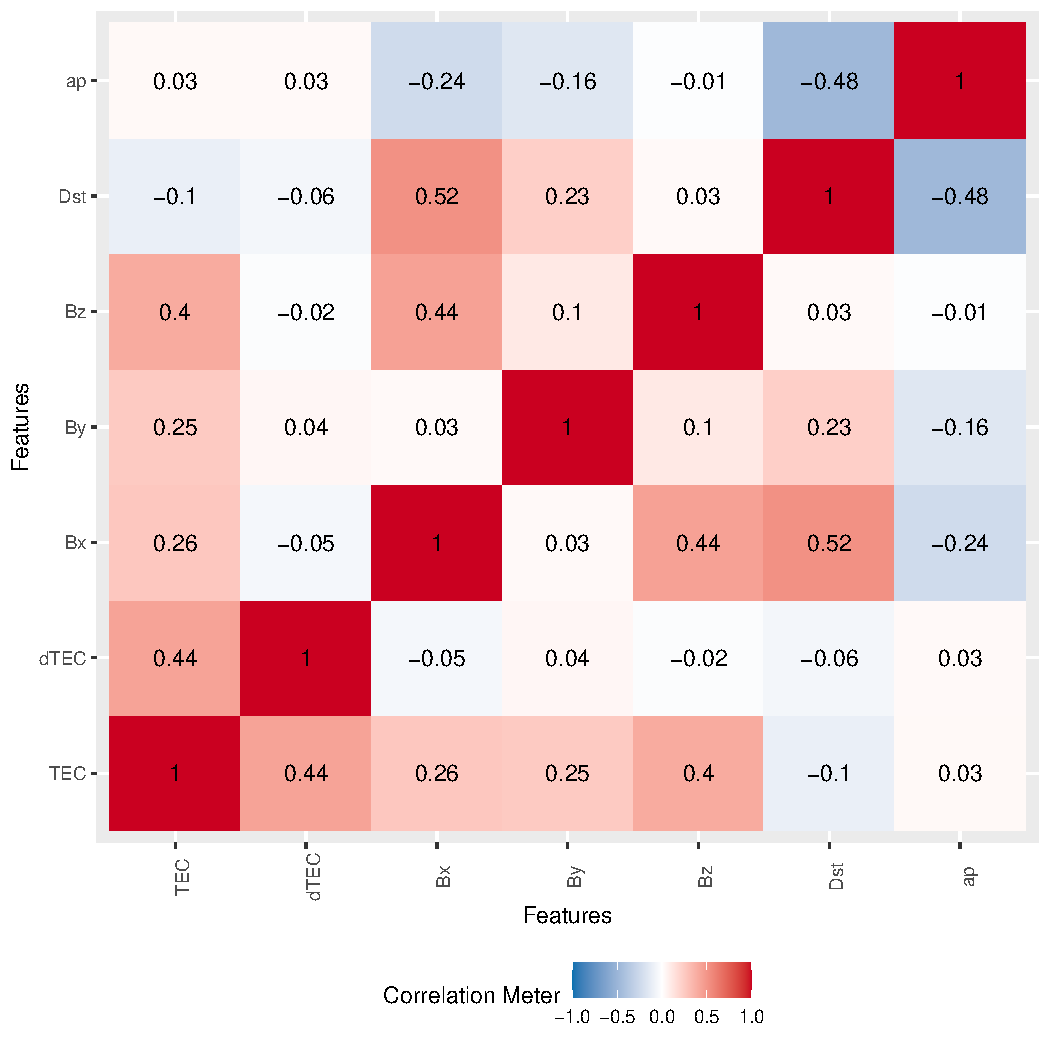
\includegraphics[width=0.9\linewidth]{iono3correlation.pdf}
    \caption{A heat map of the correlation between all variables used in this study, when the $TEC$ is less than $300$ $nT$. Red represents a high positive correlation, blue represents a high negative correlation, and white represents a low correlation. Variables are fully correlated with themselves, so values on the secondary diagonal equal $1$. The matrix is symmetrical concerning the secondary diagonal because the same combination of correlated variables is achieved when swapping the row and column.}
    \label{fig:correlation}
\end{figure}

The box plots of all variables for different ranges of $Dst$ values in Figure~\ref{fig:iono3boxplot} demonstrate that the minimum, maximum, and arithmetic mean of $a_{p}$ decrease for larger $Dst$. The opposite is true for $B_{x}$, as indicated by a high correlation in Figure~\ref{fig:correlation}. $B_{y}$ exhibits a reverse trend when compared to $B_{x}$, but it is less prominent. $B_{z}$ is the most stable with the smallest changes related to $Dst$ when observing $B_{x}$, $B_{y}$, and $B_{z}$.

\begin{figure}
    \centering
    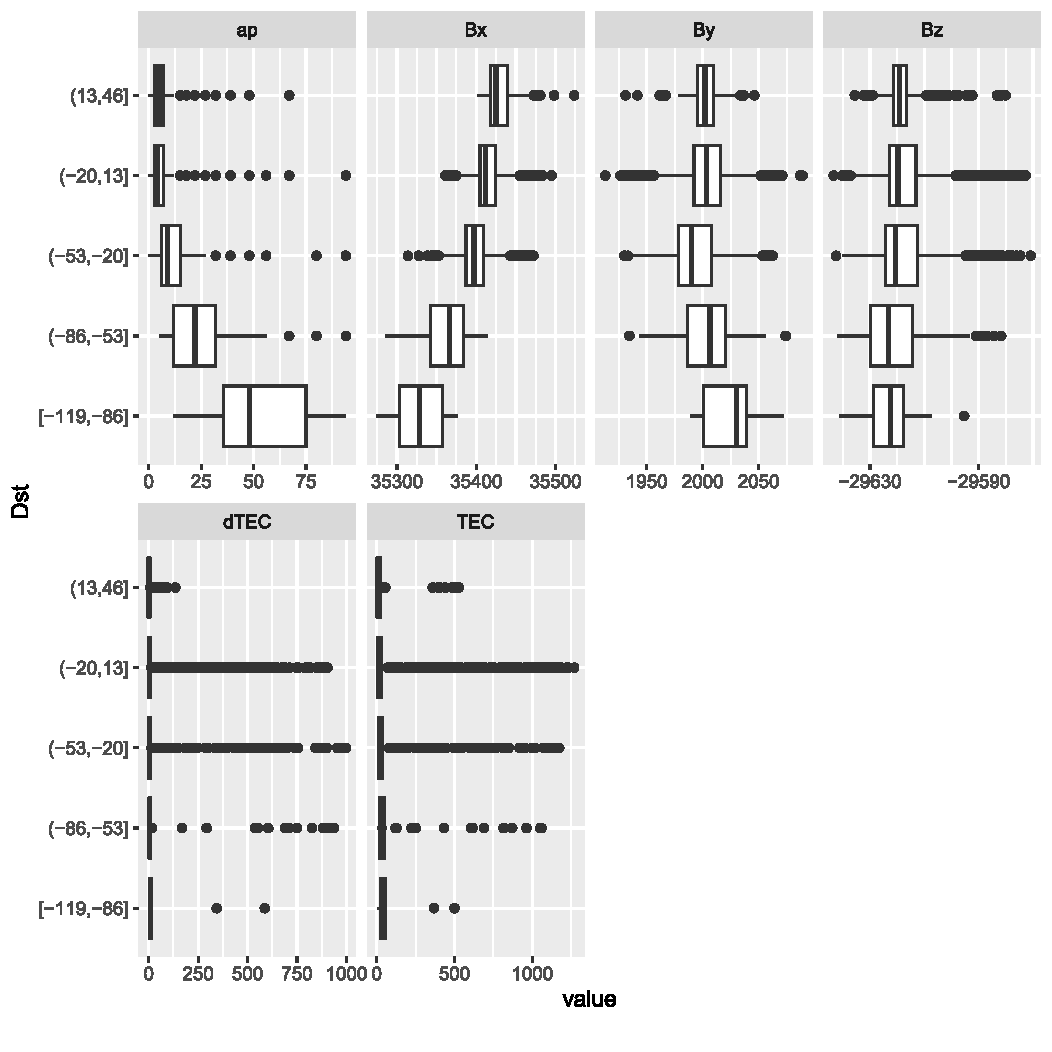
\includegraphics[width=0.9\linewidth]{iono3boxplot_fix.pdf}
    \caption{Box plots of all variables, when the $TEC$ is less than $300$ $nT$, for different ranges of $Dst$ values defining the class label used in this study.}
    \label{fig:iono3boxplot}
\end{figure}

Table~\ref{tab:minmax} provides the minimum, $1^{st}$ quartile, median, arithmetic mean, $3^{rd}$ quartile, and maximum values for all variables when the $TEC$ is less than $300$ $nT$. These values suggest that variables are not normally distributed. The Kolmogorov-Smirnov and Shapiro-Wilk normality tests, using \textit{R} functions \textit{ks.test} (ks.test developers, 2024) and \textit{shapiro.test} (shapiro.test developers, 2024), did not yield a $p$-value larger than the selected $\alpha$-value of $0.05$ for any variable, further strengthening the claim that variables do not follow a normal (Gaussian) distribution. 

\begin{table}[!ht]
    \centering
    \caption{The minimum, $1^{st}$ quartile, median, arithmetic mean, $3^{rd}$ quartile, and maximum values for all variables when the $TEC$ is less than $300$ $nT$.}
    \label{tab:minmax}
        \begin{tabular}{|c|c|c|c|c|c|c|c|}
                \hline
                  & $TEC$ & $dTEC$ & $B_{x}$ & $B_{y}$ & $B_{z}$ & $Dst$ & $a_{p}$ \\ \hline
                Min. & $1.76$ & $0.02$ & $35275.0$ & $1913.0$ & $-29649.0$ & $-119.0$ & $0.0$ \\ \hline
                $1^{st}$ Qu. & $8.43$ & $1.12$ & $35402.0$ & $1990.0$ & $-29623.0$ & $-18.0$ & $4.0$ \\ \hline
                Median & $22.83$ & $2.47$ & $35410.0$ & $2004.0$ & $-29620.0$ & $-5.0$ & $6.0$ \\ \hline
                Mean & $24.62$ & $6.208$ & $35413.0$ & $2003.0$ & $-29617.0$ & $-9.678$ & $7.539$ \\ \hline
                $3^{rd}$ Qu. & $34.23$ & $5.54$ & $35423.0$ & $2018.0$ & $-29614.0$ & $-1.0$ & $7.0$ \\ \hline
                Max. & $288.0$ & $997.0$ & $35524.0$ & $2089.0$ & $-29571.0$ & $46.0$ & $94.0$ \\ \hline
        \end{tabular}
\end{table}

\subsection{Performance Metrics}
%\label{subsec:Metrics}

The metrics and terminology used to evaluate the classifier performance were taken from the confusion matrix defined in the \textit{R} function \textit{confusionMatrix} in the \textit{caret} library (Kuhn, 2008, confusionMatrix developers, 2024).

The examples for each performance metric use only two groups (Yes and No, positive and negative). For multiple classes, results are calculated by a "one versus all" approach, viewing each class as positive and all others as negative.

\subsubsection{Confusion Matrix}
%\label{subsubsec:ConfusionMatrix}

A True Positive (TP), or True Negative (TN) result in the confusion matrix correctly indicates that the sample belongs to a class. A False Positive (FP), or False Negative (FN) classification result incorrectly claims that the sample belongs to a class and represents a type I or type II error, respectively.

Sensitivity, recall, hit rate, or True Positive Rate (TPR), calculated as $\mathrm{TP}/(\mathrm{TP}+\mathrm{FN})$, and specificity, selectivity, or True Negative Rate (TNR), calculated as $\mathrm{TN}/(\mathrm{TN}+\mathrm{FP})$, represent the proportion of correctly classified samples among those that truly belong to a class (Altman & Bland, 1994a, Altman & Bland, 1994b).

Precision, or Positive Predictive Value (PPV), calculated as $\mathrm{TP}/(\mathrm{TP}+\mathrm{FP})$, and Negative Predictive Value (NPV), calculated as $\mathrm{TN}/(\mathrm{TN}+\mathrm{FN})$, represent the proportion of correctly classified samples among those classified to a class.

Prevalence, calculated as $(\mathrm{TP}+\mathrm{FN})/(\mathrm{TP}+\mathrm{FP}+\mathrm{FN}+\mathrm{TN})$, and Detection Prevalence (DP), calculated as $(\mathrm{TP}+\mathrm{FP})/(\mathrm{TP}+\mathrm{FP}+\mathrm{FN}+\mathrm{TN})$ represent the proportion of samples that truly belong to or are classified to each class, respectively. Prevalence values other than an even split by the number of classes indicate a class imbalance.

The Detection Rate (DR), calculated as $\mathrm{TP}/(\mathrm{TP}+\mathrm{FP}+\mathrm{FN}+\mathrm{TN})$, and accuracy (Acc), calculated as $(\mathrm{TP} + \mathrm{TN}) / (\mathrm{TP} + \mathrm{TN} + \mathrm{FP} + \mathrm{FN})$, represent the proportion of correctly classified samples for separate classes or any class, respectively.

Since accuracy is unusable for unbalanced classes, Balanced Accuracy (BA)  (Velez et al., 2007) is calculated as $(\mathrm{TPR} + \mathrm{TNR}) / 2$ and represents the arithmetic mean of TPR and TNR, which are centered on the positive and the negative classes, respectively.

\section{Research Results}
\label{sec:Results}

The accuracy for all models when using all variables, all variables except $Dst$ (no $Dst$), all variables except $Dst$, $TEC$, and $dTEC$ (no $TEC$), only $B_{x}$, $B_{y}$, and $B_{z}$ (coord), only $B_{x}$, $B_{y}$, and $a_{p}$ ($x$ $y$ $a_{p}$), only $B_{x}$, $B_{z}$, and $a_{p}$ ($x$ $z$ $a_{p}$), or only $B_{y}$, $B_{z}$, and $a_{p}$ ($y$ $z$ $a_{p}$) as input is displayed in Table~\ref{tab:acc:all}. Accuracy results can lead to an incorrect conclusion if the dataset is unbalanced. Out of $9591$ samples for training and testing, $7495$ belonged to the largest N class, and $13$ to the smallest E class, as listed in Table~\ref{tab:Dstranges}. More comprehensive results by class are presented only for the Naive Bayes (NB) classifier, the second most successful model. The Neural Network (NN) classifier made no errors, so further discussion is redundant.

\begin{table}[!ht]
    \centering
    \caption{The accuracy for each model using different combinations of variables as input.}
	\label{tab:acc:all}
	\begin{tabular}{|c|c|c|c|c|c|c|c|}
		\hline
		Model & all & no $Dst$ & no $TEC$ & coord & $x$ $y$ $a_{p}$ & $x$ $z$ $a_{p}$ & $y$ $z$ $a_{p}$ \\ \hline
		SVM Poly & $0.7866$ & $0.7454$ & $0.7903$ & $0.7887$ & $0.7934$ & $0.7903$ & $0.7814$ \\ \hline
		C5.0 DT & $0.9995$ & $0.8529$ & $0.8581$ & $0.8404$ & $0.8508$ & $0.8367$ & $0.8211$ \\ \hline
		NB & $0.9953$ & $0.9943$ & $1$ & $1$ & $1$ & $1$ & $0.9995$ \\ \hline
		NN & $1$ & $1$ & $1$ & $1$ & $1$ & $1$ & $1$ \\ \hline
		PLS & $0.9212$ & $0.8258$ & $0.8232$ & $0.8174$ & $0.8153$ & $0.8143$ & $0.8007$ \\ \hline
		FDA & $0.9025$ & $0.8472$ & $0.8472$ & $0.8252$ & $0.8419$ & $0.8258$ & $0.7997$ \\ \hline
		PCA NN & $0.9963$ & $0.8492$ & $0.8492$ & $0.8399$ & $0.8456$ & $0.8367$ & $0.8185$ \\ \hline
	\end{tabular}
\end{table}

The execution time in seconds ($s$) utilizing the \textit{R} \textit{system.time} function (system.time developers, 2024) for each model and different combinations of variables as input is displayed in Table~\ref{tab:time:total}. The experiment was run on \textit{Windows} 11 using \textit{R Studio} version 2024.04.2+764 and \textit{R} version 4.4.1, the AMD Radeon RX 6600 Graphics Processing Unit (GPU), $16$ GB of Random Access Memory (RAM), and the AMD Ryzen 5 PRO 4650G Central Processing Unit (CPU) with $6$ cores. Execution time is significant because built-in systems for mobile devices using GNSS PNT have low computational capabilities.

\begin{table}[!ht]
	\centering
    \caption{The execution time in seconds ($s$) for each model when using different combinations of variables as input.}
	\label{tab:time:total}
	\begin{tabular}{|c|c|c|c|c|c|c|c|}
		\hline
		Model & all & no $Dst$ & no $TEC$ & coord & $x$ $y$ $a_{p}$ & $x$ $z$ $a_{p}$ & $y$ $z$ $a_{p}$ \\ \hline
		SVM Poly & $148.72$ & $330.67$ & $392.05$ & $582.47$ & $739.55$ & $670.54$ & $876.43$ \\ \hline
		C5.0 DT & $186.08$ & $670.61$ & $466.42$ & $347.16$ & $357.43$ & $330.81$ & $382.92$ \\ \hline
		NB & $206.65$ & $200.83$ & $164.03$ & $141.87$ & $143.97$ & $147.26$ & $149.87$ \\ \hline
		NN & $582.41$ & $629.67$ & $619.30$ & $587.37$ & $614.07$ & $629.48$ & $644.44$ \\ \hline
		PLS & $52.59$ & $63.48$ & $54.26$ & $36.90$ & $52.39$ & $41.92$ & $59.00$ \\ \hline
		FDA & $56.20$ & $98.11$ & $142.19$ & $144.53$ & $164.17$ & $172.64$ & $185.78$ \\ \hline
		PCA NN & $341.32$ & $422.86$ & $468.73$ & $452.75$ & $480.02$ & $495.66$ & $517.78$ \\ \hline
	\end{tabular}
\end{table}

\subsection{Comprehensive Results for the Naive Bayes Model}
%\label{subsec:ResultsNB}

The confusion matrix and the performance indicators derived from it for the Naive Bayes (NB) model, when using different combinations of variables as input, are depicted in Table~\ref{tab:cm:merged}, Table~\ref{tab:cs:reverse:all:nb}, Table~\ref{tab:cs:reverse:no_DisturbanceStormTime:nb}, and Table~\ref{tab:cs:reverse:yzap:nb}. The NB model was chosen because of a low computational load and high accuracy. The results for combinations of input variables with a $100\%$ accuracy using the NB model are ommited.

\begin{table}[!ht]
    \centering
    \caption{The confusion matrix for the Naive Bayes model when using all variables as input (left), all variables except $Dst$ as input (center), and only $B_{y}$, $B_{z}$, and $a_{p}$ as input (right).}
	\label{tab:cm:merged}
	\begin{tabular}{|c|c|c|c|c|c|c|c|c|c|c|c|c|c|c|c|}
		\hline
		 & \multicolumn{5}{|c|}{Reference - all} & \multicolumn{5}{|c|}{Reference - no $Dst$} & \multicolumn{5}{|c|}{Reference - $y$ $z$ $a_{p}$} \\ \hline
		 Pred. & E & N & P & R & T & E & N & P & R & T & E & N & P & R & T \\ \hline
		 E & $2$ & $0$ & $0$ & $0$ & $0$ & $2$ & $1$ & $0$ & $1$ & $0$ & $1$ & $0$ & $0$ & $0$ & $0$ \\ \hline
		 N & $0$ & $1492$ & $0$ & $1$ & $0$ & $0$ & $1492$ & $0$ & $1$ & $0$ & $1$ & $1499$ & $0$ & $0$ & $0$ \\ \hline
		 P & $0$ & $5$ & $27$ & $0$ & $0$ & $0$ & $4$ & $27$ & $0$ & $0$ & $0$ & $0$ & $27$ & $0$ & $0$ \\ \hline
		 R & $0$ & $2$ & $0$ & $369$ & $0$ & $0$ & $2$ & $0$ & $368$ & $1$ & $0$ & $0$ & $0$ & $371$ & $0$ \\ \hline
		 T & $0$ & $0$ & $0$ & $1$ & $18$ & $0$ & $0$ & $0$ & $1$ & $17$ & $0$ & $0$ & $0$ & $0$ & $18$ \\ \hline
	\end{tabular}
\end{table}

\begin{table}[!ht]
    \centering
    \caption{The performance indicators derived from the confusion matrix for the Naive Bayes model when using all variables as input.}
	\label{tab:cs:reverse:all:nb}
	\begin{tabular}{|c|c|c|c|c|c|}
		\hline
		 & \multicolumn{5}{c|}{Class} \\ \hline
		Statistics & E & N & P & R & T \\ \hline
		Sensitivity & $100\%$ & $99.53\%$ & $100\%$ & $99.46\%$ & $100\%$ \\ \hline
		Specificity & $100\%$ & $99.76\%$ & $99.735\%$ & $99.87\%$ & $99.9473\%$ \\ \hline
		PPV & $100\%$ & $99.93\%$ & $84.375\%$ & $99.46\%$ & $94.7368\%$ \\ \hline
		NPV & $100\%$ & $98.35\%$ & $100\%$ & $99.87\%$ & $100\%$ \\ \hline
		DR & $0.1043\%$ & $77.83\%$ & $1.408\%$ & $19.25\%$ & $0.939\%$ \\ \hline
		DP & $0.1043\%$ & $77.88\%$ & $1.669\%$ & $19.35\%$ & $0.9911\%$ \\ \hline
		BA & $100\%$ & $99.65\%$ & $99.868\%$ & $99.67\%$ & $99.9737\%$ \\ \hline
	\end{tabular}
\end{table}

\begin{table}[!ht]
    \centering
    \caption{The performance indicators derived from the confusion matrix for the Naive Bayes model when using all variables except $Dst$ as input.}
	\label{tab:cs:reverse:no_DisturbanceStormTime:nb}
	\begin{tabular}{|c|c|c|c|c|c|}
		\hline
		 & \multicolumn{5}{c|}{Class} \\ \hline
		Statistics & E & N & P & R & T \\ \hline
		Sensitivity & $100\%$ & $99.53\%$ & $100\%$ & $99.19\%$ & $94.4444\%$ \\ \hline
		Specificity & $99.8956\%$ & $99.76\%$ & $99.788\%$ & $99.81\%$ & $99.9473\%$ \\ \hline
		PPV & $50\%$ & $99.93\%$ & $87.097\%$ & $99.19\%$ & $94.4444\%$ \\ \hline
		NPV & $100\%$ & $98.35\%$ & $100\%$ & $99.81\%$ & $99.9473\%$ \\ \hline
		DR & $0.1043\%$ & $77.83\%$ & $1.408\%$ & $19.2\%$ & $0.8868\%$ \\ \hline
		DP & $0.2087\%$ & $77.88\%$ & $1.617\%$ & $19.35\%$ & $0.939\%$ \\ \hline
		BA & $99.9478\%$ & $99.65\%$ & $99.894\%$ & $99.5\%$ & $97.1959\%$ \\ \hline
	\end{tabular}
\end{table}

\begin{table}[!ht]
    \centering
    \caption{The performance indicators derived from the confusion matrix for the Naive Bayes model when using only $B_{y}$, $B_{z}$, and $a_{p}$ as input.}
	\label{tab:cs:reverse:yzap:nb}
	\begin{tabular}{|c|c|c|c|c|c|}
		\hline
		 & \multicolumn{5}{c|}{Class} \\ \hline
		Statistics & E & N & P & R & T \\ \hline
		Sensitivity & $50\%$ & $100\%$ & $100\%$ & $100\%$ & $100\%$ \\ \hline
		Specificity & $100\%$ & $99.76\%$ & $100\%$ & $100\%$ & $100\%$ \\ \hline
		PPV & $100\%$ & $99.93\%$ & $100\%$ & $100\%$ & $100\%$ \\ \hline
		NPV & $99.9478\%$ & $100\%$ & $100\%$ & $100\%$ & $100\%$ \\ \hline
		DR & $0.0522\%$ & $78.2\%$ & $1.408\%$ & $19.35\%$ & $0.939\%$ \\ \hline
		DP & $0.0522\%$ & $78.25\%$ & $1.408\%$ & $19.35\%$ & $0.939\%$ \\ \hline
		BA & $75\%$ & $99.88\%$ & $100\%$ & $100\%$ & $100\%$ \\ \hline
	\end{tabular}
\end{table}

\section{Discussion}
\label{sec:Discussion}

The Neural Network (NN) model has the highest execution time for any subset of the input variables due to its complexity and extensive training, evident from the data in Table~\ref{tab:time:total}. However, it achieved a $100\%$ accuracy, shown in Table~\ref{tab:acc:all}. The Naive Bayes (NB) model has the second highest accuracy, over $99\%$. The NB model achieved a $100\%$ accuracy, except when using all input variables, all input variables except Disturbance Storm-Time ($Dst$), or only $B_{y}$, $B_{z}$, and $a_{p}$. The difference in accuracy between the NN and the NB model is negligible, and the training time for the NN model is more than twice as long. An analysis in 2004 showed reasonable theoretical reasons for the seemingly incredible performance of NB classifiers (H. Zhang, 2004).

All other models fail to achieve an accuracy over $90\%$, except when using all input variables, including $Dst$. The $Dst$ class was derived by thresholding the continuous $Dst$ value and discretizing it by converting it to a single character, so the original $Dst$ value should not be used as model input. This labeling method explains the increase in accuracy when adding the $Dst$ input variable in all except the two best-performing models. For example, the C5.0 DT model did not consider any variable except $Dst$, indicated by a $100\%$ variable importance. The Support Vector Machine (SVM) model with a Polynomial Kernel is consistently the worst-performing for any subset of input variables, never achieving an accuracy over $80\%$. None of the models achieved an accuracy under $70\%$, so they were all moderately successful.

When studying the performance of the NB model by individual class in Table~\ref{tab:cm:merged}, Table~\ref{tab:cs:reverse:all:nb}, Table~\ref{tab:cs:reverse:no_DisturbanceStormTime:nb}, and Table~\ref{tab:cs:reverse:yzap:nb}, samples of the T class are all correctly classified except for one case, but the testing is less extensive since it is the second smallest class. Samples of the P class are all correctly classified. Samples of the R class are sometimes erroneously assigned to the N, T, or less commonly the E class. Two of the most common misclassifications were assigning samples of the N class with the highest detection rate and prevalence to the P or R classes with the third and second highest detection rate and prevalence. This is due to the largest number of samples in the N class between the P and R classes with the narrowest $Dst$ range. Samples of the N class are least often included in the E class, whose range is the furthest apart from the N class. A sample of the E class was attributed to the N class only once. The E class is the smallest with only two testing samples, which must be accounted for when interpreting these results, such as the lowest balanced accuracy of $75\%$ and sensitivity of $50\%$ when using only $B_{y}$, $B_{z}$, and $a_{p}$ as input, or the lowest positive predictive value of $50\%$ when using all variables as input.

\section{Conclusion}
\label{sec:Conclusion}

The presented study aims to classify ambient conditions of space weather events for sub-equatorial regions. Global Navigation Satellite System (GNSS) Positioning, Navigation, and Timing (PNT) performance is significantly affected by such events. It would be beneficial to warn users of a geomagnetic/ionospheric storm.

Classification models using machine learning were applied to descriptions of the geomagnetic field expressed in Total Electron Content ($TEC$) and other input data. It was assumed observations contained independent variables to generate the dependent variable representing the Disturbance Storm-Time ($Dst$) class. 

Statistical analysis confirmed that other variables change distribution based on $Dst$, not $TEC$. Continuous $Dst$ values in different ranges were converted into discrete classes based on statistics, previous theories, and research. 

An Support Vector Machine (SVM) with a Polynomial Kernel, C5.0 Decision Tree (DT), Naive Bayes (NB), Neural Network (NN), Partial Least Squares (PLS), Flexible Discriminant Analysis (FDA), and Principal Component Analysis (PCA) NN model created a $Dst$-based classification from multiple combinations of input variables.

The NB model achieved perfect accuracy for most tested combinations of input variables, and over $99\%$ in all cases. It is slightly less successful than the NN model, and the total execution time is at least two times shorter, making it more suitable for use in compact, low-performance, and low-cost portable devices such as smartphones.

\clearpage

\section{Acronyms}
\label{sec:Acronyms}

\textit{(AA)2} Ambient-Aware Application-Aligned


\\[2\baselineskip]

\textit{ANN} Artificial Neural Network


\\[2\baselineskip]

\textit{BA} Balanced Accuracy


\\[2\baselineskip]

\textit{CCA} Canonical Correlation Analysis

\textit{CI} Confidence Interval

\textit{CNN} Convolutional Neural Network

\textit{CPU} Central Processing Unit


\\[2\baselineskip]

\textit{DBSCAN} Density-Based Spatial Clustering

\textit{DP} Detection Prevalence

\textit{DR} Detection Rate

\textit{DT} Decision Tree

\textit{Dst} Disturbance Storm-Time


\\[2\baselineskip]

\textit{EOF} Empirical Orthogonal Functions

\textit{EPB} Equatorial Plasma Bubbles

\textit{EUV} Extreme ultraviolet

\textit{EVD} Eigenvalue Decomposition


\\[2\baselineskip]

\textit{FDA} Flexible Discriminant Analysis

\textit{FN} False Negative

\textit{FP} False Positive


\\[2\baselineskip]

\textit{GEC} Global Electric Current

\textit{GFZ} German Research Centre for Geosciences

\textit{GNSS} Global Navigation Satellite System

\textit{GPS} Global Positioning System

\textit{GPU} Graphics Processing Unit


\\[2\baselineskip]

\textit{ION} The Institute of Navigation


\\[2\baselineskip]

\textit{KLT} Karhunen–Loève Theorem


\\[2\baselineskip]

\textit{LDA} Linear Discriminant Analysis


\\[2\baselineskip]

\textit{MANOVA} Multivariate Analysis Of Variance

\textit{MARS} Multivariate Adaptive Regression Splines

\textit{ML} machine learning


\\[2\baselineskip]

\textit{NAS} Neural Architecture Search

\textit{NASA} National Aeronautics and Space Administration

\textit{NB} Naive Bayes

\textit{NDA} Normal Discriminant Analysis

\textit{NIR} No Information Rate

\textit{NN} Neural Network

\textit{NOAA} National Oceanic and Atmospheric Administration

\textit{NPV} Negative Predictive Value

\textit{NRCAN} Natural Resources Canada


\\[2\baselineskip]

\textit{PCA} Principal Component Analysis

\textit{PLS} Partial Least Squares

\textit{PLS-DA} Partial Least Squares Discriminant Analysis

\textit{PNT} Positioning, Navigation, and Timing

\textit{POD} Proper Orthogonal Decomposition

\textit{PPV} Positive Predictive Value


\\[2\baselineskip]

\textit{RAM} Random Access Memory

\textit{RF} Random Forest

\textit{RIN} The Royal Institute of Navigation

\textit{RINEX} Receiver Independent Exchange Format


\\[2\baselineskip]

\textit{SAR} Synthetic Aperture Radar

\textit{SPDF} Space Physics Data Facility

\textit{SVC} Support Vector Clustering

\textit{SVD} Singular Value Decomposition

\textit{SVM} Support Vector Machine

\textit{SVN} Support Vector Network

\textit{SWPC} Space Weather Prediction Center


\\[2\baselineskip]

\textit{TDIDT} Top-Down Induction of Decision Trees

\textit{TEC} Total Electron Content

\textit{TID} Traveling Ionospheric Disturbance

\textit{TN} True Negative

\textit{TNR} True Negative Rate

\textit{TP} True Positive

\textit{TPR} True Positive Rate


\\[2\baselineskip]

\textit{URSI} Union Radio-Scientifique Internationale


\\[2\baselineskip]

\textit{dTEC} standard deviation of Total Electron Content



\section{Declarations}
%\label{sec:Declarations}

\subsection{Availability of data and materials}
%\label{subsec:Availability}

The datasets used during the current study are available from the corresponding author upon reasonable request.

\subsection{Competing interests}
%\label{subsec:Competing}

The authors declare no conflict of interest.

\subsection{Funding}
%\label{subsec:Funding}

The authors have no funding sources to declare.

\subsection{Authors' contributions}
%\label{subsec:Contributions}

L\v{Z} and DK contributed to conceptualization, methodology, software, validation, formal analysis, investigation, data curation, writing of the original draft, reviewing and editing the text, and visualization. TI contributed to validation, formal analysis, investigation, review and editing, supervision, and project administration. RF contributed to conceptualization, methodology, investigation, resources, writing of the original draft, reviewing and editing the text, and supervision. All authors read and approved the final manuscript.

\subsection{Acknowledgements}
%\label{subsec:Acknowledgements}

Not applicable

\subsection{Authors' information}
%\label{subsec:Information}

LŽ is a doctoral student at the Faculty of Engineering, University of Rijeka, currently employed as an assistant at the Department of Computer Science. Her research interests include applied machine learning in biology, chemistry, medicine, and transportation. Maritime transportation is also the subject of her doctoral research.

DK is a doctoral student at the Faculty of Engineering, University of Rijeka, currently employed as an assistant at the Department of Computer Science. His research interests include applied machine learning in object recognition and image segmentation. Image classification and labeling are also the subject of his doctoral research.

TI earned his MSc and PhD in telecommunication engineering from the University of Ruse “Angel Kanchev,” Ruse, Bulgaria, in 1999 and 2007, respectively. He is a full professor at the Department of Telecommunication, University of Ruse “Angel Kanchev.” His research interests include mobile communications networks, signal processing, wireless technologies, and satellite navigation. Professor Iliev is a Member of IEEE.

RF is an external Professor of Electronics Engineering with the Department for Computer Science, Faculty of Engineering, and Center for Artificial Intelligence and Cybersecurity, both at the University of Rijeka, Croatia, and Head of the Laboratory for Spatial Intelligence at Hrvatsko Zagorje Krapina University of Applied Science, Krapina, Croatia. He holds a BSc, MSc, and PhD in electrical engineering, obtained in 1987, 1994, and 2007, respectively, from the Faculty of Electrical Engineering and Computing, University of Zagreb, Croatia. His professional interests include Ambient-Aware Application-Aligned ((AA)2) Global Navigation Satellite System (GNSS) Positioning, Navigation, and Timing (PNT), spatial uncertainty quantification, spatial statistical learning, predictive modeling, statistical signal processing, trajectory analysis and prediction, and occupancy modeling. Professor Filjar is a Fellow of The Royal Institute of Navigation (RIN) (London, United Kingdom), a Member of The Institute of Navigation (ION) (Manassas, Virginia), a Senior Member of Union Radio-Scientifique Internationale (URSI) (Ghent, Belgium) and a Member of The Society for Industrial and Applied Mathematics  (Philadelphia, Philadelphia). %He established, and organises the traditional Baška SIF (Spatial Information Fusion) Forum, held annually in Baška, Krk Island, Croatia.

% vidi Philadelphia možda clan, zemlje u razvoju samo 15 dolara godišnje, ciljane sekcije
% uncertainty modeling souther California

% smanjti reference ko je moguce

%%===========================================================================================%%
%% If you are submitting to one of the Nature Portfolio journals, using the eJP submission   %%
%% system, please include the references within the manuscript file itself. You may do this  %%
%% by copying the reference list from your .bbl file, paste it into the main manuscript .tex %%
%% file, and delete the associated \verb+\bibliography+ commands.                            %%
%%===========================================================================================%%

\section{Bibliography}
%\label{sec:Bibliography}
[1] R. Filjar, “An application-centred resilient GNSS position estimation algorithm based on positioning environment conditions awareness,” in Proceedings of the 2022 International Technical Meeting of The Institute of Navigation, 2022, pp. 1123–1136.

[2] R. Filjar, I. Hedji, J. Prpić-Oršić, and T. Iliev, “An Ambient Adaptive Global Navigation Satellite System Total Electron Content Predictive Model for Short-Term Rapid Geomagnetic Storm Events,” Remote Sensing, vol. 16, no. 16, p. 3051, 2024.

[3] K. Davies, Ionospheric Radio. Futures Place, Stevenage: Institution of Engineering & Technology, 1990. [Online] . Available: https://books.google.hr/books?id=qdWUKSj5PCcC

[4] M. Filić and R. Filjar, “modelling the relation between GNSS positioning performance degradation, and space weather and ionospheric conditions using RReliefF features selection,” in ION GNSS+ 2018 Meeting, 2018, pp. 1999–2006.

[5] J. J. Spilker Jr, P. Axelrad, B. W. Parkinson, and P. Enge, Global positioning system: theory and applications, volume I. Reston, Virginia: American Institute of Aeronautics, 1996.

[6] A. Oxley, Uncertainties in GPS Positioning: A mathematical discourse. Cambridge, Massachusetts: Academic Press, 2017.

[7] G. K. Seemala, “Chapter 4 - Estimation of ionospheric total electron content (TEC) from GNSS observations,” in Atmospheric Remote Sensing, A. Kumar Singh and S. Tiwari, Eds. Amsterdam, Netherlands: Elsevier, 2023, pp. 63–84. doi: https://doi.org/10.1016/B978-0-323-99262-6.00022-5.

[8] N. Sikirica, F. Dimc, O. Jukic, T. B. Iliev, D. Spoljar, and R. Filjar, “A Risk Assessment of Geomagnetic Conditions Impact on GPS Positioning Accuracy Degradation in Tropical Regions Using Dst Index,” in Proceedings of the 2021 International Technical Meeting of The Institute of Navigation, 2021, pp. 606–615.

[9] R. Natras, B. Soja, and M. Schmidt, “Ensemble machine learning of random forest, AdaBoost and XGBoost for vertical total electron content forecasting,” Remote Sensing, vol. 14, no. 15, p. 3547, 2022.

[10] R. Natras et al., “Regional ionosphere delay models based on CORS data and machine learning,” NAVIGATION: Journal of the Institute of Navigation, vol. 70, no. 3, 2023.

[11] NOAA, NOAA Space Weather Scales | NOAA / NWS Space Weather Prediction Center — swpc.noaa.gov. https://www.swpc.noaa.gov/noaa-scales-explanation, 2024. [Online] . Available: https://www.swpc.noaa.gov/noaa-scales-explanation

[12] R. Filjar, I. Sklebar, and M. Horvat, “A COMPARISON OF MACHINE LEARNING-BASED INDIVIDUAL MOBILITY CLASSIFICATION MODELS DEVELOPED ON SENSOR READINGS FROM LOOSELY ATTACHED SMARTPHONES.,” Komunikácie, vol. 22, no. 4, 2020.

[13] INTERMAGNET and others, Intermagnet reference data set (IRDS) 2019 – definitive magnetic observatory data. GFZ Data Services, 2022. doi: https://doi.org/10.5880/INTERMAGNET.1991.2019.

[14] M. Kuhn, Applied predictive modeling. Springer, 2013.

[15] M. Kuhn, The caret Package — topepo.github.io. https://topepo.github.io/caret/, 2024. [Online] . Available: https://topepo.github.io/caret/

[16] RCoreTeam, R: The R Project for Statistical Computing — r-project.org. https://www.r-project.org/, 2024. [Online] . Available: https://www.r-project.org/

[17] C. Cortes and V. Vapnik, “Support-vector networks,” Mach. Learn., vol. 20, no. 3, pp. 273–297, Sep. 1995.

[18] P. scikit-learn developers, 1.4. Support Vector Machines — scikit-learn.org. http://scikit-learn.org/stable/modules/svm.html, 2023. [Online] . Available: http://scikit-learn.org/stable/modules/svm.html

[19] B. E. Boser, I. M. Guyon, and V. N. Vapnik, “A training algorithm for optimal margin classifiers,” Jul. 1992.

[20] M. A. Aizerman, E. A. Braverman, and L. Rozonoer, “Theoretical foundations of the potential function method in pattern recognition learning,” in Automation and Remote Control, 1964, no. 25, pp. 821–837.

[21] T. Hastie, S. Rosset, J. Zhu, and H. Zou, “Multi-class AdaBoost,” Stat. Interface, vol. 2, no. 3, pp. 349–360, 2009.

[22] A. Ben-Hur, D. Horn, H. Siegelmann, and V. Vapnik, “Support Vector Clustering,” Journal of Machine Learning Research, vol. 2, pp. 125–137, Nov. 2001, doi: 10.1162/15324430260185565.

[23] D. Meyer, F. Leisch, and K. Hornik, “The support vector machine under test,” Neurocomputing, vol. 55, no. 1–2, pp. 169–186, Sep. 2003.

[24] C. Jin and L. Wang, “Dimensionality dependent PAC-Bayes margin bound,” Advances in Neural Information Processing Systems, vol. 2, pp. 1034–1042, Jan. 2012.

[25] W. H. Press, S. A. Teukolsky, W. T. Vetterling, and B. P. Flannery, Numerical recipes 3rd edition, Third. Cambridge, England: Cambridge University Press, 2007.

[26] C. W. Hsu, C. C. Chang, and C. J. Lin, “A Practical Guide to Support Vector Classification,” Department of Computer Science, National Taiwan University, techreport, 2003.

[27] L. Rokach and O. Maimon, Data mining with decision trees. Singapore: World Scientific Publishing Company, 2014.

[28] M. Studer, G. Ritschard, A. Gabadinho, and N. S. Müller, “Discrepancy analysis of state sequences,” Sociol. Methods Res., vol. 40, no. 3, pp. 471–510, Aug. 2011.

[29] X. Wu et al., “Top 10 algorithms in data mining,” Knowl. Inf. Syst., vol. 14, no. 1, pp. 1–37, Jan. 2008.

[30] S. Shalev-Shwartz and S. Ben-David, “Decision Trees,” in Understanding Machine Learning: From Theory to Algorithms, Cambridge, England: Cambridge University Press, 2014, pp. 212–218. doi: 10.1017/CBO9781107298019.019.

[31] J. R. Quinlan, “Induction of decision trees,” Mach. Learn., vol. 1, no. 1, pp. 81–106, Mar. 1986.

[32] L. Rokach and O. Maimon, “Top-down induction of decision trees classifiers—A survey,” IEEE Trans. Syst. Man Cybern. C Appl. Rev., vol. 35, no. 4, pp. 476–487, Nov. 2005.

[33] D. J. Hand and K. Yu, “Idiot’s Bayes: Not So Stupid after All?,” Int. Stat. Rev., vol. 69, no. 3, p. 385, Dec. 2001.

[34] A. McCallum, Graphical Models Lecture 2: Bayesian Network Representation. https://people.cs.umass.edu/ mccallum/courses/gm2011/02-bn-rep.pdf, 2011. [Online] . Available: https://people.cs.umass.edu/ mccallum/courses/gm2011/02-bn-rep.pdf

[35] S. J. Russell and P. Norvig, Artificial intelligence: a modern approach. London, England: Pearson, 2016.

[36] V. Metsis, I. Androutsopoulos, and G. Paliouras, “Spam Filtering with Naive Bayes - Which Naive Bayes?,” Jan. 2006.

[37] R. Caruana and A. Niculescu-Mizil, “An Empirical Comparison of Supervised Learning Algorithms,” Proceedings of the 23rd international conference on Machine learning - ICML ’06, vol. 2006, pp. 161–168, Jun. 2006, doi: 10.1145/1143844.1143865.

[38] G. H. John and P. Langley, Estimating Continuous Distributions in Bayesian Classifiers. 2013.

[39] A. Mccallum and K. Nigam, “A Comparison of Event Models for Naive Bayes Text Classification,” Work Learn Text Categ, vol. 752, May 2001.

[40] M. N. Murty and V. S. Devi, Pattern recognition: An algorithmic approach. Berlin/Heidelberg, Germany: Springer Science & Business Media, 2011.

[41] MIT, Explained: Neural networks — news.mit.edu. https://news.mit.edu/2017/explained-neural-networks-deep-learning-0414, 2017. [Online] . Available: https://news.mit.edu/2017/explained-neural-networks-deep-learning-0414

[42] A. Brahme, Comprehensive biomedical physics. 8-11 Southampton Street, London: Newnes, 2014.

[43] J. D. Olden and D. A. Jackson, “Illuminating the ‘black box’: a randomization approach for understanding variable contributions in artificial neural networks,” Ecological modelling, vol. 154, no. 1–2, pp. 135–150, 2002.

[44] S. L. Özesmi and U. Özesmi, “An artificial neural network approach to spatial habitat modelling with interspecific interaction,” Ecological modelling, vol. 116, no. 1, pp. 15–31, 1999.

[45] C. Bishop, Pattern Recognition and Machine Learning. Berlin/Heidelberg, Germany: Springer, 2006.

[46] V. Vapnik, The nature of statistical learning theory. Berlin/Heidelberg, Germany: Springer science & business media, 2013.

[47] I. Goodfellow, Deep learning. MIT press, 2016.

[48] P. Probst, A. L. Boulesteix, and B. Bischl, “Tunability: Importance of hyperparameters of machine learning algorithms,” Journal of Machine Learning Research, vol. 20, no. 53, pp. 1–32, 2019.

[49] K. Pearson, “LIII. On lines and planes of closest fit to systems of points in space,” The London, Edinburgh, and Dublin philosophical magazine and journal of science, vol. 2, no. 11, pp. 559–572, 1901.

[50] F. M. Stewart, Introduction to linear algebra. Mineola, New York, USA: Courier Dover Publications, 2019.

[51] I. T. Jolliffe and J. Cadima, “Principal component analysis: a review and recent developments,” Philosophical transactions of the royal society A: Mathematical, Physical and Engineering Sciences, vol. 374, no. 2065, p. 20150202, 2016.

[52] B. D. Ripley, Pattern recognition and neural networks. Cambridge, United Kingdom: Cambridge university press, 2007.

[53] S. Wold, M. Sjöström, and L. Eriksson, “PLS-regression: a basic tool of chemometrics,” Chemometrics and intelligent laboratory systems, vol. 58, no. 2, pp. 109–130, 2001.

[54] H. Abdi, “Partial least squares regression and projection on latent structure regression (PLS Regression),” Wiley interdisciplinary reviews: computational statistics, vol. 2, no. 1, pp. 97–106, 2010.

[55] S. Sæbø, T. Almøy, A. Flatberg, A. H. Aastveit, and H. Martens, “LPLS-regression: a method for prediction and classification under the influence of background information on predictor variables,” Chemometrics and Intelligent Laboratory Systems, vol. 91, no. 2, pp. 121–132, 2008.

[56] F. Lindgren, P. Geladi, and S. Wold, “The kernel algorithm for PLS,” Journal of Chemometrics, vol. 7, no. 1, pp. 45–59, 1993.

[57] S. De Jong and C. J. F. Ter Braak, “Comments on the PLS kernel algorithm,” Journal of chemometrics, vol. 8, no. 2, pp. 169–174, 1994.

[58] B. S. Dayal and J. F. MacGregor, “Improved PLS algorithms,” Journal of Chemometrics: A Journal of the Chemometrics Society, vol. 11, no. 1, pp. 73–85, 1997.

[59] S. De Jong, “SIMPLS: an alternative approach to partial least squares regression,” Chemometrics and intelligent laboratory systems, vol. 18, no. 3, pp. 251–263, 1993.

[60] S. Rännar, F. Lindgren, P. Geladi, and S. Wold, “A PLS kernel algorithm for data sets with many variables and fewer objects. Part 1: Theory and algorithm,” Journal of Chemometrics, vol. 8, no. 2, pp. 111–125, 1994.

[61] Y. Takane and S. Loisel, “On the PLS algorithm for multiple regression (PLS1),” in The Multiple Facets of Partial Least Squares and Related Methods: PLS, Paris, France, 2014 8, 2016, pp. 17–28.

[62] A. Höskuldsson, “PLS regression methods,” Journal of chemometrics, vol. 2, no. 3, pp. 211–228, 1988.

[63] R. A. Fisher, “The use of multiple measurements in taxonomic problems,” Annals of eugenics, vol. 7, no. 2, pp. 179–188, 1936.

[64] G. J. McLachlan, Discriminant analysis and statistical pattern recognition. Hoboken, New Jersey, U.S.: John Wiley & Sons, 2005.

[65] T. Hastie, A. Buja, and R. Tibshirani, “Penalized discriminant analysis,” The Annals of Statistics, vol. 23, no. 1, pp. 73–102, 1995.

[66] T. Hastie, R. Tibshirani, J. H. Friedman, and J. H. Friedman, The elements of statistical learning: data mining, inference, and prediction, vol. 2. Berlin/Heidelberg, Germany: Springer, 2009.

[67] T. Hastie, R. Tibshirani, and A. Buja, “Flexible discriminant analysis by optimal scoring,” Journal of the American statistical association, vol. 89, no. 428, pp. 1255–1270, 1994.

[68] C. Reynès, R. Sabatier, and N. Molinari, “Choice of B-splines with free parameters in the flexible discriminant analysis context,” Computational statistics & data analysis, vol. 51, no. 3, pp. 1765–1778, 2006.

[69] N. D. Phillips et al., “Applying species distribution modelling to a data poor, pelagic fish complex: the ocean sunfishes,” Journal of biogeography, vol. 44, no. 10, pp. 2176–2187, 2017.

[70] W. Hallgren, F. Santana, S. Low-Choy, Y. Zhao, and B. Mackey, “Species distribution models can be highly sensitive to algorithm configuration,” Ecological Modelling, vol. 408, p. 108719, 2019.

[71] W. Thuiller, D. Georges, R. Engler, and F. Breiner, “Ensemble platform for species distribution modeling,” R Package Version, pp. 3–1, 2016.

[72] P. Quillfeldt, J. O. Engler, J. R. D. Silk, and R. A. Phillips, “Influence of device accuracy and choice of algorithm for species distribution modelling of seabirds: a case study using black-browed albatrosses,” Journal of Avian Biology, vol. 48, no. 12, pp. 1549–1555, 2017.

[73] Z. Zhang, S. Xu, C. Capinha, R. Weterings, and T. Gao, “Using species distribution model to predict the impact of climate change on the potential distribution of Japanese whiting Sillago japonica,” Ecological Indicators, vol. 104, pp. 333–340, 2019.

[74] D. Wetcher-Hendricks, Analyzing quantitative data: An introduction for social researchers. Hoboken, New Jersey, U.S.: John Wiley & Sons, 2011.

[75] J. Cohen, P. Cohen, S. G. West, and L. S. Aiken, Applied multiple regression/correlation analysis for the behavioral sciences. Milton Park, Abingdon-on-Thames, Oxfordshire, England, UK: Routledge, 2013.

[76] G. D. Garson, PA 765: Discriminant Function Analysis — web.archive.org. https://web.archive.org/web/20080312065328/http://www2.chass.ncsu.edu/garson/pA765/discrim.htm, 2008. [Online] . Available: https://web.archive.org/web/20080312065328/http://www2.chass.ncsu.edu/garson/pA765/discrim.htm

[77] C. R. Rao, “The utilization of multiple measurements in problems of biological classification,” Journal of the Royal Statistical Society. Series B (Methodological), vol. 10, no. 2, pp. 159–203, 1948.

[78] J. Hansen, Using SPSS for windows and macintosh: analyzing and understanding data. Taylor & Francis, 2005.

[79] J. A. Klobuchar, “Design and characteristics of the GPS ionospheric time delay algorithm for single frequency users,” in PLANS 1986-Position Location and Navigation Symposium, 1986, pp. 280–286.

[80] B. Zolesi and Lj. R. Cander, Ionospheric prediction and forecasting. Berlin/Heidelberg, Germany: Springer, 2014.

[81] A. Komjathy, “Global ionospheric total electron content mapping using the Global Positioning System,” University of New Brunswick, Department of Geodesy, techreport, 1997. [Online] . Available: https://api.semanticscholar.org/CorpusID:128511894

[82] NOAA, HF Radio Communications | NOAA / NWS Space Weather Prediction Center — swpc.noaa.gov. http://www.swpc.noaa.gov/impacts/hf-radio-communications, 2024. [Online] . Available: http://www.swpc.noaa.gov/impacts/hf-radio-communications

[83] S. Kotz, N. Balakrishnan, C. B. Read, B. Vidakovic, and N. L. Johnson, Encyclopedia of Statistical Sciences, Volume 1. Hoboken, New Jersey, U.S.: John Wiley & Sons, 2005.

[84] P. I. Vellinov, C. W. Spassov, and S. I. Kolev, “Ionospheric effects of lightning during the increasing part of solar cycle 22,” Journal of atmospheric and terrestrial physics, vol. 54, no. 10, pp. 1347–1353, 1992.

[85] M. Liu, G. Luo, and H. Wang, “The 2013 Lushan earthquake in China tests hazard assessments,” Seismological Research Letters, vol. 85, no. 1, pp. 40–43, 2014.

[86] M. Ulukavak and M. Yalcinkaya, “Analysis of ionospheric anomalies due to space weather conditions by using GPS-TEC variations,” in FIG Congress, 2018, pp. 6–11.

[87] R. Schwenn, “Solar wind: Global properties,” in Encyclopedia of Astronomy & Astrophysics, Boca Raton, Florida, USA: CRC Press, 2001, pp. 1–9.

[88] V. F. Melnikov, “Relationships between Microwave, Hard X ray, and Corpuscular Emissions of Solar Flares,” phdthesis, Ph. D. Thesis, Radiophysical Research Institute, Nizhniy Novgorod, Russia, 1990.

[89] A. P. I. Android developers, Sensor types | Android Open Source Project — source.android.com. https://source.android.com/docs/core/interaction/sensors/sensor-types#magnetic_field_sensor, 2024. [Online] . Available: https://source.android.com/docs/core/interaction/sensors/sensor-types#magnetic_field_sensor

[90] M. H. De Canck, “Ionosphere properties and behaviors,” Antennex, vol. 119, pp. 6–7, 2007.

[91] NOAA, swpc.noaa.gov. https://www.swpc.noaa.gov/sites/default/files/images/u2/TheK-index.pdf, 2024. [Online] . Available: https://www.swpc.noaa.gov/sites/default/files/images/u2/TheK-index.pdf

[92] J. Matzka, Kp Index — gfz-potsdam.de. https://www.gfz-potsdam.de/en/section/geomagnetism/data-products-services/geomagnetic-kp-index, 2024. [Online] . Available: https://www.gfz-potsdam.de/en/section/geomagnetism/data-products-services/geomagnetic-kp-index

[93] NOAA, Alerts, Watches and Warnings | NOAA / NWS Space Weather Prediction Center — swpc.noaa.gov. https://www.swpc.noaa.gov/products/alerts-watches-and-warnings, 2024. [Online] . Available: https://www.swpc.noaa.gov/products/alerts-watches-and-warnings

[94] N. Papitashvili, SPDF - About OMNIWeb Data — omniweb.gsfc.nasa.gov. http://omniweb.gsfc.nasa.gov/html/ow_data.html, 2024. [Online] . Available: http://omniweb.gsfc.nasa.gov/html/ow_data.html

[95] N. Papitashvili, OMNIWeb Data Explorer — omniweb.gsfc.nasa.gov. http://omniweb.gsfc.nasa.gov/form/dx1.html, 2024. [Online] . Available: http://omniweb.gsfc.nasa.gov/form/dx1.html

[96] L. M. M. Myint, K. Hozumi, S. Saito, and P. Supnithi, “Analysis of local geomagnetic index under the influence of equatorial electrojet (EEJ) at the equatorial Phuket geomagnetic station in Thailand,” Advances in Space Research, vol. 70, no. 5, pp. 1429–1440, 2022, doi: https://doi.org/10.1016/j.asr.2022.06.024.

[97] NOAA, swpc.noaa.gov. https://www.swpc.noaa.gov/sites/default/files/images/NOAAscales.pdf, 2024. [Online] . Available: https://www.swpc.noaa.gov/sites/default/files/images/NOAAscales.pdf

[98] J. Matzka, O. Bronkalla, K. Tornow, K. Elger, and C. Stolle, Geomagnetic Kp index. GFZ Data Services, 2021. doi: https://doi.org/10.1016/j.asr.2022.06.024.

[99] J. Matzka, C. Stolle, Y. Yamazaki, O. Bronkalla, and A. Morschhauser, The geomagnetic KP index and derived indices of geomagnetic activity, vol. 19. American Geophysical Union (AGU), 2021. doi: https://doi.org/10.1029/2020SW002641.

[100] NOAA, Geomagnetic kp and ap Indices | NCEI — ngdc.noaa.gov. https://www.ngdc.noaa.gov/stp/GEOMAG/kp_ap.html, 2024. [Online] . Available: https://www.ngdc.noaa.gov/stp/GEOMAG/kp_ap.html

[101] C. A. Loewe and G. W. Prölss, “Classification and mean behavior of magnetic storms,” Journal of Geophysical Research: Space Physics, vol. 102, no. A7, pp. 14209–14213, 1997.

[102] W. D. Gonzalez et al., “What is a geomagnetic storm?,” Journal of Geophysical Research: Space Physics, vol. 99, no. A4, pp. 5771–5792, 1994.

[103] Y. Kamide et al., “Two-step development of geomagnetic storms,” Journal of Geophysical Research: Space Physics, vol. 103, no. A4, pp. 6917–6921, 1998.

[104] A. Rozhnoi, M. S. Solovieva, O. A. Molchanov, and M. Hayakawa, “Middle latitude LF (40 kHz) phase variations associated with earthquakes for quiet and disturbed geomagnetic conditions,” Physics and Chemistry of the Earth, Parts A/B/C, vol. 29, no. 4–9, pp. 589–598, 2004.

[105] M. E. Contadakis, D. N. Arabelos, C. Pikridas, and S. D. Spatalas, “Total electron content variations over southern Europe before and during the M 6.3 Abruzzo earthquake of April 6, 2009,” Annals of geophysics, vol. 55, no. 1, 2012.

[106] M. Kuhn, 4 Data Splitting | The caret Package — topepo.github.io. https://topepo.github.io/caret/data-splitting.html, 2024. [Online] . Available: https://topepo.github.io/caret/data-splitting.html

[107] R. J. Hyndman, Forecasting: principles and practice. Melbourne, Australia: OTexts, 2018.

[108] R. createDataPartition developers, createDataPartition function - RDocumentation — rdocumentation.org. https://www.rdocumentation.org/packages/caret/versions/6.0-94/topics/createDataPartition, 2024. [Online] . Available: https://www.rdocumentation.org/packages/caret/versions/6.0-94/topics/createDataPartition

[109] R. E. Fan, K. W. Chang, C. J. Hsieh, X. R. Wang, and C. J. Lin, “LIBLINEAR: a library for large linear classification,” Journal of Machine Learning Research, vol. 9, pp. 1871–1874, Aug. 2008, doi: 10.1145/1390681.1442794.

[110] I. B. Mohamad and D. Usman, “Standardization and its effects on K-means clustering algorithm,” Research Journal of Applied Sciences, Engineering and Technology, vol. 6, no. 17, pp. 3299–3303, Sep. 2013.

[111] P. G. Fennell, Z. Zuo, and K. Lerman, “Predicting and explaining behavioral data with structured feature space decomposition,” EPJ Data Sci., vol. 8, no. 1, Dec. 2019.

[112] R. ks.test developers, ks.test function - RDocumentation — rdocumentation.org. https://www.rdocumentation.org/packages/stats/versions/3.6.2/topics/ks.test, 2024. [Online] . Available: https://www.rdocumentation.org/packages/stats/versions/3.6.2/topics/ks.test

[113] R. shapiro.test developers, shapiro.test function - RDocumentation — rdocumentation.org. https://www.rdocumentation.org/packages/stats/versions/3.6.2/topics/shapiro.test, 2024. [Online] . Available: https://www.rdocumentation.org/packages/stats/versions/3.6.2/topics/shapiro.test

[114] M. Kuhn, “Building predictive models in R using the caret package,” Journal of statistical software, vol. 28, pp. 1–26, 2008.

[115] R. confusionMatrix developers, confusionMatrix function - RDocumentation — rdocumentation.org. https://www.rdocumentation.org/packages/caret/versions/6.0-94/topics/confusionMatrix, 2024. [Online] . Available: https://www.rdocumentation.org/packages/caret/versions/6.0-94/topics/confusionMatrix

[116] D. G. Altman and J. M. Bland, “Diagnostic tests. 1: Sensitivity and specificity.,” BMJ: British Medical Journal, vol. 308, no. 6943, p. 1552, 1994.

[117] D. G. Altman and J. M. Bland, “Diagnostic test 2: predictive values,” BMJ: British Medical Journal, vol. 309, p. 102, 1994.

[118] D. R. Velez et al., “A balanced accuracy function for epistasis modeling in imbalanced datasets using multifactor dimensionality reduction,” Genetic Epidemiology: the Official Publication of the International Genetic Epidemiology Society, vol. 31, no. 4, pp. 306–315, 2007.

[119] R. system.time developers, system.time function - RDocumentation — rdocumentation.org. https://www.rdocumentation.org/packages/base/versions/3.6.2/topics/system.time, 2024. [Online] . Available: https://www.rdocumentation.org/packages/base/versions/3.6.2/topics/system.time

[120] H. Zhang, “The Optimality of Naive Bayes,” in Proceedings of the Seventeenth International Florida Artificial Intelligence Research Society Conference, FLAIRS 2004, Jan. 2004, vol. 2.


\end{document}